\documentclass[preprint,12pt]{elsarticle}

\usepackage{graphicx}
\usepackage{booktabs}
\usepackage{amsmath}
\usepackage{amssymb}
\usepackage{tabularx}
\usepackage{microtype}
\usepackage{placeins}
\usepackage{hyperref}
\hypersetup{hidelinks}

\graphicspath{{figures/}}

% Allow floats near their call sites (default [t]-only queues them to the end).
\renewcommand{\topfraction}{0.9}
\renewcommand{\bottomfraction}{0.8}
\renewcommand{\textfraction}{0.07}
\renewcommand{\floatpagefraction}{0.65}
\setcounter{topnumber}{4}
\setcounter{bottomnumber}{3}
\setcounter{totalnumber}{6}

% Soften overfull lines from bold / monospace runs without ragged paragraphs.
\emergencystretch=2.5em
\tolerance=1500

% Center a tabular; scale down only if it would overflow the text width.
\newsavebox{\wsfitbox}
\newcommand{\fitcenter}[1]{%
  \sbox{\wsfitbox}{#1}%
  \centering
  \ifdim\wd\wsfitbox>\linewidth
    \resizebox{\linewidth}{!}{\usebox{\wsfitbox}}%
  \else
    \usebox{\wsfitbox}%
  \fi
}

% Wide diagrams (Fig.~1 / Fig.~3): prefer full text width.
\newcommand{\pagefitfig}[1]{%
  \includegraphics[width=\linewidth,height=0.55\textheight,keepaspectratio]{#1}%
}

\journal{Swarm and Evolutionary Computation}

% Fill these at journal submission (after tagging the release commit on GitHub).
\newcommand{\SubmissionGitTag}{journal-v1}
\newcommand{\SubmissionGitShort}{TBD} % e.g. 7607364b4d31 — replace with `git rev-parse --short=12 HEAD` of the tagged commit
\newcommand{\SubmissionGitFull}{TBD}  % full 40-char SHA of the same commit

% Drop elsarticle "Preprint submitted to …" footer (Elsevier EM preference).
\makeatletter
\def\ps@pprintTitle{%
  \let\@oddhead\@empty
  \let\@evenhead\@empty
  \def\@oddfoot{\reset@font\hfil\thepage\hfil}%
  \let\@evenfoot\@oddfoot
}
\makeatother

\begin{document}

\begin{frontmatter}

\title{Two Roles for Surrogates in {LLM}-Guided {MAP}-{E}lites: Before- vs.\ After-Generation Surrogates}

\author{Artem Starovoitov\corref{cor1}}
\ead{artem.starovoitov@proton.me}
\ead[url]{https://orcid.org/0009-0005-3170-4865}
\address{Independent Engineer, Moscow, Russia}
\cortext[cor1]{Corresponding author}

\begin{abstract}
Previous LLM-guided and surrogate-assisted QD work often compares \emph{pipelines} (different emitters, policies, and surrogate use bundled together). We compare \emph{attachment points}: where the same surrogate enters a propose$\rightarrow$evaluate loop, holding checkpoint, archive, budget, and emitters fixed. In LLM-guided MAP-Elites that yields a before-generation surrogate vs.\ an after-generation surrogate (Figure~\ref{fig:pipeline}; synonyms once in \S\ref{sec:terminology}). \textbf{Takeaway:} only the after-generation attach role shows a measurable evaluation-efficiency gain ($\sim$3.7~pp coverage per simulation at 15k--20k evaluations; 33.5\% fewer sims at fixed iterations; Figure~\ref{fig:acquisition})---not a terminal-coverage or wall-clock win on this evaluator ($-0.83$~pp; $\sim$20 vs.\ $\sim$7~min). Matched-policy before-generation (H1) stays within $\pm 2$~pp (TOST at $n{=}10$; MDE$\approx$1.2~pp). A historical bundled $+15$~pp contrast is confounded (\S\ref{sec:decomposition}). Stacking both under LLM (H3) stays \textbf{exploratory}: we diagnose a dual compose-gate definition (offline hold-out vs.\ live filter), localize divergent skip to a $74.6\%$ gray band, and report honest NMAE degradation after target alignment (\S\ref{sec:h3}, \S\ref{sec:limitations})---without a new confirmatory run in this version. After-generation AUC also ports to a dungeon factorial (H5) and, on an interim maze slice ($n{=}5$ five-arm; $n{=}10$ CPU H2 pair), to a third domain with the same partial pattern (filter ports; LLM does not). Magnitudes are testbed-specific; caveats in \S\ref{sec:limitations}.
\end{abstract}

\begin{keyword}
quality-diversity \sep MAP-Elites \sep large language models \sep surrogate-assisted optimization \sep open-ended search
\end{keyword}

\end{frontmatter}

\section{Introduction}

Quality-diversity (QD) algorithms maintain archives of solutions that are both high-performing and behaviourally diverse. MAP-Elites assigns each candidate to a behavioural niche and keeps the best elite per cell~\cite{mouret2015illuminating}. Every candidate still needs a black-box evaluation; when that roll-out is costly, evaluation count dominates wall time and surrogate-assisted illumination becomes attractive~\cite{gaier2018sail}.

LLMs are increasingly used as variation operators in QD loops: they edit structured genotypes and emit semantically meaningful mutations. An LLM-guided MAP-Elites stack therefore couples an LLM (or hybrid) emitter, a simulator that buys ground truth, and an archive. The LLM does not observe simulator outcomes unless the loop feeds feedback into the prompt; a surrogate is a natural place to inject that feedback---but \emph{where} it attaches is usually confounded with the rest of the stack.

Previous work often compared complete \emph{pipelines} (emitters, archive policies, and surrogate use bundled together). We compare \textbf{attachment points}. Holding one shared checkpoint, matched emitters, archive, and budget fixed, we ask whether a before-generation surrogate (prompt-side scalars) or an after-generation surrogate (hard evaluation gate) moves archive metrics (Figure~\ref{fig:pipeline}). Payoffs are measured on a controlled black-box evaluator (\S\ref{sec:substrate}), not studied as a domain contribution. Labels \textbf{H1}--\textbf{H5} name the contrasts (Table~\ref{tab:role-exp}).

\subsection{Contributions}

\begin{enumerate}
  \item \textbf{Attachment-point decomposition.} Previous work compared pipelines; we compare where the same surrogate attaches---before vs.\ after generation---with the rest of the stack held fixed (Figure~\ref{fig:pipeline}; \S\ref{sec:decomposition}--\ref{sec:h2}).
  \item \textbf{Bundled ``hints'' lift is mostly not hint content.} A locked stub$\rightarrow$hints contrast looks large ($\approx{+}15$~pp) but confounds archive policy with surrogate use. At matched \texttt{uniform\_frontier}, policy alone recovers $\approx{+}14.8$~pp; live prompt scalars vs.\ stub constants stay within $\pm 2$~pp (H1; $n{=}10$; post-hoc TOST).
  \item \textbf{Only after-generation attachment (H2) improves evaluation efficiency.} Threshold gating without an LLM gains $\sim$3.7~pp coverage per simulation at 15k--20k evaluations and skips 33.5\% of sims (Figure~\ref{fig:acquisition})---not a terminal-coverage or wall-clock win on this cheap evaluator.
  \item \textbf{Stacking under LLM (H3) is exploratory.} The locked production filter fails compose-gate skip agreement; we localize the mismatch and defer a gray-zone repair (\S\ref{sec:h3}).
  \item \textbf{Placement ports more readily than bundled LLM lift.} After-generation AUC transfers to dungeon (and interim maze) domains; genetic MAP-Elites still leads LLM arms there (H5).
\end{enumerate}

Section~\ref{sec:method} defines the loop and attach roles; \S\ref{sec:protocol} the confirmatory design; \S\ref{sec:results} follows H1$\rightarrow$H2$\rightarrow$H3, then H4/H5; \S\ref{sec:discussion} separates architecture from payoff. Caveats and deferred work: \S\ref{sec:limitations}.

\section{Background and related work}
\label{sec:related}

\subsection{Quality-diversity and MAP-Elites}

Quality-diversity (QD) algorithms seek collections of high-performing yet behaviourally diverse solutions rather than a single optimum~\cite{pugh2016quality,cully2018quality,chatzilygeroudis2021qd}. MAP-Elites maintains an archive partitioned by user-defined behavioural characteristics (BC) and retains the best elite per niche~\cite{mouret2015illuminating}. Heterogeneous emitter sets can improve illumination efficiency relative to a single variation operator~\cite{cully2020multiemitter}; our confirmatory stack mixes random, genetic, and LLM slots in one batch.

Continuous variation operators remain important on fixed-length genomes. Covariance Matrix Adaptation MAP-Elites (CMA-ME) couples CMA-ES adaptation with MAP-Elites archiving and often dominates random or isotropic mutation on continuous control and design tasks~\cite{fontaine2020cmame}. CMA-MAE extends the idea with MAP-annealing and separate result archives, trading coverage for per-niche quality~\cite{fontaine2023cmamae,zhao2024cmamae}. We implement both through \texttt{ribs} v0.11.0~\cite{pyribs2020} with an adapter that evaluates candidates on the same black-box simulator as the LLM stack (\S\ref{sec:method}). Our pyribs baselines use homogeneous CMA-ES emitter pools rather than mixed pyribs ``cocktails,'' so they represent strong but not maximal pyribs configurations.

\subsection{Surrogate-assisted illumination}

Expensive simulators motivate surrogate models that predict outcomes from static design features~\cite{jin2005fitness,jones1998ego}.
Classical surrogate-assisted evolutionary algorithms (SAEAs) treat that prediction problem as \emph{model management}: when, and how strongly, to trust the approximate fitness instead of the true evaluator~\cite{jin2005fitness}.
Two recurring evolution-control patterns are \emph{individual-based} control (pre-select or filter candidates before expensive evaluation) and \emph{generation-based} control (evaluate only some generations fully, or alternate approximate and exact generations).
Our before-/after-generation split is an LLM-guided MAP-Elites instance of that same dilemma, not a QD-only invention.
The after-generation surrogate is individual-based pre-selection: a threshold gate decides whether a proposed genome spends a simulator call.
The before-generation surrogate is a softer, non-controlling use of the same model---surrogate scalars enter the LLM prompt and try to shape variation, but never skip \texttt{evaluate\_candidate}.
That soft channel is closer to model-informed operators than to classical hard evolution control; our matched H1 result (prompt scalars flat once archive policy is fixed) is therefore readable as evidence that soft model advice is easy for a constrained LLM emitter to ignore, whereas hard individual-based gating reallocates evaluations (\S\ref{sec:decomposition}--\ref{sec:h2}).

Surrogate-Assisted Illumination (SAIL) is the canonical QD answer: fit a Gaussian process over the behaviour--fitness landscape, run MAP-Elites on an acquisition surface (classically UCB-style), and spend real evaluations only on a selected subset~\cite{gaier2018sail,gaier2017sail,gaier2017aiaa}.
Deep Surrogate Assisted MAP-Elites (DSA-ME) replaces the GP with neural predictors trained online in an inner loop and validates candidates in an outer game-engine loop~\cite{grillotti2022dsame}.
Related Bayesian QD lines couple acquisition to descriptor and fitness models~\cite{kent2025boqd}.
Discount Model Search continues the surrogate-QD line without LLMs, replacing histogram discounts with a learned continuous discount model for high-dimensional measure spaces~\cite{tjanaka2026dms}.
Across this QD family the surrogate is a \emph{search accelerator}: it can change which candidates receive ground truth, and often \emph{is} the surface being illuminated rather than a side channel into an otherwise unchanged MAP-Elites loop.
SAIL-style acquisition is thus a strong form of individual-based evolution control specialized to behaviour--fitness GPs; our after-generation threshold gate is SAIL-\emph{kin} in that controlling sense, while the before-generation prompt channel has no direct SAIL analogue.

Reported evaluation savings are strongest in computational design.
On two-dimensional airfoil tasks SAIL needs orders-of-magnitude fewer flow simulations than MAP-Elites while filling behaviour bins~\cite{gaier2018sail}; with the budget CMA-ES requires to optimize one bin, SAIL can match that quality in every bin~\cite{gaier2017sail}.
Three-dimensional aerodynamics and high-dimensional discrete deckbuilding show the same qualitative pattern~\cite{gaier2017aiaa,grillotti2022dsame}.
Evidence for stochastic simulators is thinner: these studies assume expensive but largely deterministic evaluators or batched outer validation, not single-rollout archive updates under seeded simulator noise.
Our confirmatory tier holds the simulator budget fixed (32{,}500 evaluations per seed) and asks, for LLM-guided QD, \emph{where} the same surrogate should attach under full-simulation archive updates---not whether a new SAIL-style illuminator brand wins on expensive CFD.

\textbf{Positioning vs.\ SAIL / DSA-ME.}
Our stack differs from those lineages on four points that matter for the before/after framework.
(i)~\emph{Model:} a multi-task MLP ensemble with MC-dropout over genome features (optional LightGBM path), not a monolithic GP fitness surface; an offline hold-out ablation at runtime-aligned gate~$0.95$ still prefers the production MLP over a sklearn GP on composed fitness ($R^2{=}0.94$ / NMAE$=0.112$ vs.\ $0.89$ / $0.222$; ${\sim}37\times$ faster) and rejects GP+UCB as a drop-in acquisition upgrade (\S\ref{sec:acquisition}). A legacy gate-$0.5$ snapshot ($R^2{=}0.76$ vs.\ ${\approx}0.22$) is not a valid model-quality contrast (\S\ref{sec:checkpoint}).
(ii)~\emph{Attach points:} the before-generation surrogate \textbf{never skips} \texttt{evaluate\_candidate}---it only supplies scalars to the LLM prompt---while the after-generation surrogate optionally gates with a production \texttt{threshold\_gate} ($\texttt{min\_fit}{=}0.45$, $\texttt{max\_u}{=}1.0$), not SAIL's GP-UCB illuminator.
(iii)~\emph{Truth vs.\ guidance:} prompt fitness is recomposed from predicted components with the same closed form as the simulator (Eq.~\eqref{eq:fitness}), but archive insertion always uses simulated metrics; DSA-ME's online inner/outer split is closer to the after-generation surrogate than to the before-generation surrogate, yet still does not inject surrogate text into an LLM emitter.
(iv)~\emph{Disclosure:} we report a diagnosed compose-gate dual-definition (offline hold-out vs.\ live filter), its impact on surrogate validity metrics (NMAE degradation after alignment), and gray-zone localization of blocked H3---transparency that SAIL-style papers rarely need when fitness definitions stay matched end-to-end.
We therefore treat SAIL/DSA-ME as related surrogate-QD lineages rather than drop-in baselines; pyribs CMA-ME/CMA-MAE (\S\ref{sec:pyribs}) are the quantitative QD baselines for this protocol.

\subsection{LLMs in evolutionary and QD search}

LLMs have been used as variation operators, prompt optimizers, and evolutionary engines~\cite{wu2025ecllm,wang2025llmea,vanstein2024llamea,guo2024evoprompt,liu2024llmeo,lange2024llmes}. Program-search lines pair a frozen LLM with an external evaluator to evolve code or rewards (FunSearch; Eureka)~\cite{romera2024funsearch,ma2024eureka}; Promptbreeder evolves task and mutation prompts self-referentially~\cite{fernando2024promptbreeder}; OpenELM surveys open-ended LLM evolution~\cite{lehman2023openelm}. Closest to our QD setting, LLMatic couples LLM code generation with CVT-MAP-Elites for neural architecture search~\cite{nasir2024llmatic}, and in-context QD generators sample diverse solutions from LLM priors~\cite{lim2024llmqd}. Behaviour-space analyses of LLaMEA further compare dual-prompt mutation strategies on anytime search dynamics~\cite{vanstein2025behaviour}. Concurrent LLM+MAP-Elites applications include D{\'e}j{\`a}Q's learnability-guided curation of RL-with-verifiable-rewards datasets~\cite{ropke2026dejaq} and medical decision-pipeline evolution without a surrogate/gating layer~\cite{sviridov2026medical}---both use LLM variation in a QD loop, but neither treat before- vs.\ after-generation surrogates as an experimental factor. Procedural-content pipelines apply evolutionary search and LLMs to level generators and structured genotypes~\cite{togelius2010sbpcg,earle2022nca}; emitters must respect simulators that validate and repair invalid outputs (as in our dungeon domain, \S\ref{sec:results}). Open-ended CA worlds have likewise been illuminated with QD archives~\cite{faldor2024lenia}.

A complementary line treats the \emph{prompt itself} as the search space: Diverse Prompts applies MAP-Elites over prompt phenotypes for BigBench Lite tasks~\cite{santos2025diverseprompts}, evolutionary sampling explores instruction diversity more broadly~\cite{saletta2024promptspace}, and parameter-efficient neuroevolution steers frozen LLMs by evolving prompt embeddings rather than using the LLM as a genotype emitter~\cite{guo2026qdllm}. Those settings illuminate prompts (or embeddings) for a fixed downstream LLM call, whereas we mutate \texttt{WorldSpec} genomes and inject simulator-derived \emph{surrogate scalars} into the mutation prompt. A different surrogate use keeps the LLM on fitness estimation: LLM-assisted evolutionary algorithms (LAEA) and related LLM-driven SAEAs prompt a model to classify or regress candidate quality~\cite{hao2024laea,xie2025llmsae}. We instead pair a genome-aligned ML regressor (trained on simulator logs) with an LLM \emph{emitter} that edits structured genotypes---the LLM is \emph{not} the surrogate.

\subsection{Seeded simulators and uncertain QD}

Prior LLM+QD systems often evaluate on deterministic or batched offline tasks. Our confirmatory evaluations are \emph{deterministically seeded} from the genotype (canonical SHA-256), so re-evaluating the same candidate reproduces the same fitness and BC even when the underlying simulator rules are stochastic. Elites are therefore not lucky-seed artifacts in the UQD sense.

Uncertain QD (UQD) formalizes the complementary setting where fitness and BC are distributions and archive policies re-sample to limit lucky outliers~\cite{flageat2023uq,flageat2025extractqd,flageat2025tradeoff}. We do \emph{not} claim that confirmatory results stress-test UQD: every inserted elite uses a single seeded pass, and tests use paired experiment seeds with Holm correction on terminal coverage and mean elite fitness (\S\ref{sec:protocol}). We separate \emph{archive truth} (always simulated) from \emph{emitter guidance} (before- and/or after-generation surrogates). Archive target-selection policy is orthogonal to those two surrogate roles. UQD methods remain relevant if future work disables canonical seeding or budgets multiple independent rollouts per niche.

Table~\ref{tab:positioning} summarizes how the present work relates to the closest prior clusters.

\begin{table}[!htbp]
  \centering
  \caption{Positioning vs.\ related QD + surrogate + LLM lines.}
  \label{tab:positioning}
  \small
  \fitcenter{%
  \begin{tabular}{@{}llp{3.2cm}l@{}}
    \toprule
    Line & Surrogate & LLM role & Skip real eval? \\
    \midrule
    Classical SAEA model mgmt.\cite{jin2005fitness} & Approx.\ fitness; individual / generation control & --- & Often (pre-selection) \\
    SAIL / DSA-ME & GP / deep predictor as search surface & --- & Often yes \\
    LAEA / LLM-SAEA & LLM \emph{as} fitness model & Surrogate / ranker & Sometimes \\
    LLMatic & --- & Code/variation emitter & No (NAS training) \\
    Prompt-aug.\ LLM search & Text advice (often none) & Mutator / coder & Usually no \\
    \textbf{This work} & Offline MLP/GBM (shared); H1 soft / H2 hard & structured genotype mutator; roles compared & Optional (H2) \\
    \bottomrule
  \end{tabular}%
  }
\end{table}

\noindent\textit{Key difference from SAIL:} we do not replace MAP-Elites search with a GP acquisition illuminator; we ask \emph{where} a fixed MLP checkpoint attaches in an LLM-guided propose$\rightarrow$evaluate loop, and we gate with a fitness threshold rather than UCB over a GP surface (\S\ref{sec:acquisition}). The after-generation surrogate is intentionally SAIL-\emph{kin} and classical individual-based pre-selection (hard evaluation gate); the before-generation surrogate is the soft, non-controlling channel (prompt scalars that never skip simulation) that makes the before/after comparison non-redundant with SAIL-style illumination alone.
\textit{Key difference from DSA-ME:} predictors are an offline shared checkpoint feeding an optional before-generation surrogate and after-generation skips, not an online inner-loop illuminator with outer game-engine validation.
\textit{Key difference from LAEA:} the LLM never estimates fitness---the MLP does; the LLM only proposes structured genomes.
\textit{Key difference from classical SAEA generation-based control:} we do not alternate approximate vs.\ exact \emph{generations}; both H1 and H2 operate per candidate slot inside a fixed MAP-Elites batch schedule.

\section{Method}
\label{sec:method}

We study an LLM-guided MAP-Elites propose$\rightarrow$evaluate loop with a shared surrogate that can attach as a before-generation surrogate or an after-generation surrogate. Figure~\ref{fig:pipeline} is the architectural map; the evaluator is a measurement substrate only (\S\ref{sec:substrate}). Archive fitness always comes from the simulator---the surrogate never replaces ground truth for insertion.

\begin{figure}[!htbp]
  \centering
  \pagefitfig{fig01_pipeline.pdf}
  \caption{Architectural attach-role map for LLM-guided MAP-Elites: \emph{before-generation surrogate} (H1) vs.\ \emph{after-generation surrogate} (H2). Stacking both under LLM (H3) is an exploratory interaction path.}
  \label{fig:pipeline}
\end{figure}

\subsection{Attachment points and contrast labels}
\label{sec:terminology}

A MAP-Elites iteration is select $\rightarrow$ \textbf{generate} $\rightarrow$ (optionally) gate $\rightarrow$ \textbf{evaluate} $\rightarrow$ archive update. Surrogate knowledge can intervene at two moments (Figure~\ref{fig:pipeline}):

\begin{itemize}
  \item \textbf{Before-generation surrogate} --- predictions enter the emitter and try to change \emph{what} is proposed (never skips simulation).
  \item \textbf{After-generation surrogate} --- predictions gate the candidate and change \emph{whether} it spends ground truth (SAIL-\emph{kin} hard gate).
\end{itemize}

We use those two names throughout. Synonyms appear only here: before-generation $\equiv$ prompt hints / guidance; after-generation $\equiv$ acquisition / candidate filtering. Table~\ref{tab:role-exp} maps attach points to reader labels \textbf{H1}--\textbf{H5}. Prompt placeholders and thresholds are mechanisms \emph{inside} a role. Surrogate-informed parent selection is out of scope; archive \texttt{target\_selection} remains ordinary MAP-Elites policy.

\begin{table}[!htbp]
  \centering
  \caption{Where the surrogate attaches $\leftrightarrow$ which contrast speaks to it.}
  \label{tab:role-exp}
  \small
  \fitcenter{%
  \begin{tabular}{@{}llll@{}}
    \toprule
    Integration point & Experiment & Label & Status \\
    \midrule
    Before-generation & \texttt{stub\_uniform} vs.\ \texttt{hints} & H1 & exploratory (TOST$\pm$2~pp) \\
    After-generation & \texttt{genetic\_me\_uniform} vs.\ \texttt{genetic\_me\_filter} & H2 & eval-efficiency gain \\
    Both under LLM & \texttt{hints} vs.\ \texttt{filter} & H3 & exploratory (compose-gate blocked) \\
    Continuous-relaxation ref.\ & hints vs.\ cma\_me / cma\_mae & H4 & protocol control (does not pass) \\
    Cross-domain transfer & dungeon + maze AUC & H5 & partial (H2 ports; LLM does not) \\
    \bottomrule
  \end{tabular}%
  }
\end{table}

The bundled stub/hints contrast mixes archive policy with surrogate use and is \emph{not} H1 (appendix Table~\ref{tab:families}). Shared-checkpoint hold-out validity is a gate before H1--H3, not a separate H-label.

\subsection{MAP-Elites illuminator loop}

Each run executes \texttt{iterations} $\times$ \texttt{batch\_size} candidate slots in fixed order. Production schedulers use $650 \times 50 = 32{,}500$ simulator calls per seed. For slot~$k$ the loop:
\begin{enumerate}
  \item selects a target niche (behaviour-cell centre) according to \texttt{target\_selection};
  \item calls the slot emitter (\texttt{random}, \texttt{genetic}, or \texttt{llm}) to propose a \texttt{WorldSpec};
  \item optionally applies surrogate acquisition (\S\ref{sec:acquisition});
  \item runs \texttt{evaluate\_candidate} $\rightarrow$ \texttt{run\_world} (always for accepted slots in MVP hint mode);
  \item inserts into the archive if fitness strictly improves the cell incumbent;
  \item appends training data to the surrogate buffer when \texttt{surrogate.enabled}.
\end{enumerate}
LLM slots log \texttt{llm\_fallback} when parsing fails and a genetic repair path is used. Parallel evaluation uses a process pool sized to the batch; LLM emit uses up to four concurrent HTTP workers per iteration. Outputs: \texttt{map\_elites\_archive.jsonl}, optional \texttt{archive\_trace.jsonl}, and \texttt{nightly\_run\_summary.json}.

\textbf{Target selection (not a surrogate role).} \texttt{min\_fitness\_frontier} picks the occupied cell with lowest elite fitness (used by the bundled \texttt{stub} arm). \texttt{uniform\_frontier} samples uniformly among occupied cells (used by \texttt{hints}, filter arms, and matched H1/H2 controls). These are archive policies over occupied niches; they do \emph{not} use the surrogate to select parents. H1 holds this policy fixed (\S\ref{sec:decomposition}). Surrogate-assisted parent/niche selection is out of scope here.

\subsection{Surrogate model}
\label{sec:surrogate-method}

The surrogate maps a canonical \texttt{WorldSpec} to predicted MAP-Elites outcomes without a simulator call (Figure~\ref{fig:surrogate}). Feature schema~2.1 encodes 24 genome-aligned dimensions (discrete rule bits and continuous scalars; \S\ref{sec:substrate}). A multi-head regressor (\textbf{Strategy~A}) predicts seven component targets---stability, diversity, oscillation, two topology proxies, final density, and early-extinction probability---trained from JSONL buffer rows appended after each real evaluation when the surrogate is enabled.

Production checkpoint \texttt{nightly\_v3\_mc\_d005.pkl} is a four-member MLP ensemble with MC-dropout uncertainty ($N=35{,}114$ training rows; hold-out at runtime-aligned compose gate~$0.95$: $R^2_{\text{fitness}}=0.94$ [95\% CI $0.94{,}0.95$], MAE$_{\text{fitness}}=0.029$, NMAE$=0.112$; \S\ref{sec:checkpoint}). Runtime fitness is recomposed via \texttt{compute\_fitness\_from\_prediction} using Eq.~\eqref{eq:fitness} (same weights as the simulator). \texttt{get\_surrogate()} falls back to constant \texttt{StubSurrogate} values if the checkpoint is missing, dimension-mismatched, or fails the \texttt{hints\_ok} gate ($R^2 \ge 0.30$, MAE $< 0.085$).

\textbf{Before-generation surrogate (H1).} Before each LLM call, \texttt{SurrogateFacade.predict(parent)} runs on the \emph{parent} elite's spec. Placeholders \texttt{\{surrogate\_mean\}} and \texttt{\{surrogate\_uncertainty\}} in the user prompt receive \texttt{prediction.fitness} and calibrated ensemble spread. When \texttt{surrogate.enabled=false}, fixed YAML stubs (\texttt{stub\_mean}, \texttt{stub\_uncertainty}) are substituted without calling \texttt{predict}. One LLM HTTP request per LLM slot regardless of surrogate mode.

\subsection{LLM emitter}

The \texttt{LlmEmitter} sends the parent \texttt{WorldSpec} JSON and niche centre to a chat-completions API; the model returns a JSON patch applied via \texttt{world\_spec\_from\_llm}. Stack~v2 uses temperature~0.2, \texttt{max\_tokens=350}, and \texttt{llm\_parallel\_workers=4}. Primary LLM runs use Alibaba \texttt{qwen-turbo} (DashScope); multi-provider replications swap provider YAML while keeping prompts and schedulers fixed (\S\ref{sec:results}). Model IDs are window-pinned in run summaries (\texttt{llm\_spec\_hash}); floating endpoint aliases are disclosed per provider.

Accepted LLM elites typically differ from parents by structured rule-table and scalar edits rather than bit noise (qualitative parent diffs on \texttt{hints}; appendix~\S\ref{sec:substrate-appendix}). That supports calling LLM variation \emph{semantic} without claiming a QD win once target selection is matched.

\subsection{After-generation surrogate (H2)}
\label{sec:acquisition}

Optional \texttt{acquisition.mode=filter} evaluates \texttt{surrogate.predict} \emph{before} \texttt{evaluate\_candidate}. A \texttt{threshold\_gate} skips simulation when predicted fitness falls below \texttt{min\_predicted\_fitness=0.45} (primary grid) subject to uncertainty calibration. Skipped slots are logged to \texttt{surrogate\_archive.jsonl} but do not update the MAP-Elites archive. \texttt{shadow} mode logs counterfactual skips while still evaluating.

\textbf{Why MLP + threshold gate, not SAIL-style GP+UCB.}
We use an MLP ensemble with MC-dropout uncertainty and a fitness threshold gate ($\texttt{min\_fit}{=}0.45$, $\texttt{max\_u}{=}1.0$), rather than a SAIL-style GP+UCB acquisition.
On the nightly buffer hold-out at the \emph{runtime-aligned} compose gate~$0.95$, the production MLP achieves $R^2{=}0.94$ (NMAE$=0.112$) vs.\ $0.89$ (NMAE$=0.222$) for a scikit-learn GP fitness regressor trained on 5{,}000 rows under the \emph{same} label definition, and is ${\sim}37\times$ faster at a 32{,}500-proposal batch.
An earlier M1 snapshot at misaligned gate~$0.5$ reported MLP $R^2{=}0.76$ vs.\ GP ${\approx}0.22$; that gap is not reusable as a model-quality argument because ${\approx}96\%$ of gate-$0.5$ labels are zero (\S\ref{sec:checkpoint}).
The aligned comparison still prefers MLP on $R^2$, NMAE, and latency, but the margin is narrower.
Offline acquisition replay shows that replacing the MLP with the GP under the \emph{same} threshold gate worsens the false-skip proxy ($0.7\%\!\rightarrow\!3.2\%$); a UCB skip rule on GP scores ($\mu{+}\beta\sigma < \texttt{min\_fit}$, $\beta\in\{0.15,0.5,1.0\}$) stays near $99\%$ skip and does not improve false-skip.
On logged Q1 filter proposals ($n{=}325{,}000$), replaying UCB on the \emph{same} MLP $\mu/\sigma$ only softens the gate (skip $33.5\%\!\rightarrow\!28.5\%/25.7\%/21.2\%$) and never adds skips---still without claiming an online QD win for UCB.
With $\texttt{max\_u}{=}1.0$, uncertainty is not load-bearing for the production threshold gate.
We therefore treat GP+UCB as a related SAIL lineage, not a competitive drop-in for this stack (artifact: \texttt{artifacts/surrogate/gp\_ucb\_ablation.json}).

The locked compose-gate check on historical production \texttt{filter} remains \textbf{blocked} ($d{=}0.528$ at $\tau{=}0.45$), but offline replay diagnoses the mechanism (dual gate; $74.6\%$ gray band; \S\ref{sec:h3}). A protocol amendment (2026-07-28) aligns hold-out compose to production ($0.95$) and pre-specifies a deferred gray-zone repair arm (\texttt{filter\_gray\_zone} vs.\ \texttt{hints}; journal extension). H3 on the locked production arm stays exploratory in this version. H2 reports matched \texttt{genetic\_me\_uniform} vs.\ \texttt{genetic\_me\_filter} as the primary filter evidence (\S\ref{sec:h2}).

\subsection{pyribs CMA-ME / CMA-MAE baselines}
\label{sec:pyribs}

Gradient QD baselines run through \texttt{run\_pyribs\_baseline.py} (\texttt{ribs==0.11.0}), \emph{not} as native \texttt{EmitterKind} types. The adapter maps the same 21-D genetic genome to \texttt{WorldSpec}, evaluates with the same simulator as the LLM stack, and writes comparable JSONL archives. Each algorithm uses \textbf{five homogeneous} \texttt{EvolutionStrategyEmitter} instances (batch~50 each $\Rightarrow$ ask size~250 per generation), initial step size $\sigma_0=0.2$, and 32{,}500 total evaluations. CMA-ME uses learning rate~1.0 with 2-improvement ranking and filter selection; CMA-MAE uses learning rate~0.01, improvement ranking, and a separate result archive. This is a strong but not maximal pyribs configuration (no mixed ImprovementEmitter / RandomDirectionEmitter cocktail). We treat pyribs comparisons as cross-pipeline references alongside the in-repo heterogeneous MAP-Elites stack---same honesty bar as the continuous-relaxation caveat: encoding and initialization are disclosed below, not hidden advantages.

\textbf{Encoding (continuous relaxation; apples-to-oranges caveat).}
CMA's \texttt{EvolutionStrategyEmitter} proposes continuous $\theta\in\mathbb{R}^{21}$; \texttt{decode\_genome} then \emph{rints} the 18 rule bits and clips the three scalars before simulation. Genetic / LLM emitters, by contrast, edit discrete rule tables (and named scalars) directly. The comparison is therefore \emph{not} bit-identical variation: CMA searches a continuous relaxation of a mixed discrete/continuous genotype, where covariance adaptation can exploit local structure that bit-flip genetics never sees. We treat the pyribs arms as an \textbf{upper-bound style ceiling for continuous-friendly representations} of this genome---not as a fair discrete-vs-discrete duel. A discrete CMA-style emitter is \emph{implementable} in pyribs via a custom \texttt{EmitterBase}; we run three supplementary controls (\S\ref{sec:h4}): \textbf{Bernoulli-decode} CMA-ME (package~C4; continuous proposal, discrete bits at eval), a \textbf{native bit-flip} \texttt{DiscreteCMAEmitter} (\texttt{q1-v3-pyribs-native-discrete-cma}), and \textbf{pbCMA} (\texttt{q1-v3-pyribs-pbcma}; latent Gaussian CMA + bit threshold + margin; discrete genotype in archive). Decode/cold-start ablation shows the hints$\ll$CMA gap survives alternate \emph{continuous} decodes; C4 and pbCMA both lead hints by $\sim$10~pp; native discrete confirms a smaller $+5.2$~pp margin. pbCMA closes most of the native$\rightarrow$Bernoulli gap ($+4.4$~pp vs.\ native; $-1.3$~pp vs.\ Bernoulli) but still trails \texttt{rint} ($-3.4$~pp), so full continuous-relaxation encoding retains a modest edge beyond latent covariance adaptation alone.

\textbf{Warm-start (symmetric).} All confirmatory primary-grid arms---\texttt{vanilla}, genetic ME variants, \texttt{stub}/\texttt{hints}/\texttt{filter}, and pyribs CMA-ME/MAE---load the \emph{same} nightly grid baseline JSONL ($\sim$2{,}614 elites) via \texttt{--load-archive} before the 32{,}500-evaluation budget. Terminal coverage is reported after warm-start merge/collapse. The pyribs contrast is matched on initialization as well as evaluation count; asymmetries arise from emitter pipelines and continuous-relaxation encoding, not from unequal archive seeds.

\begin{figure}[!htbp]
  \centering
  \pagefitfig{fig03_surrogate_flow.pdf}
  \caption{Shared surrogate detail: schema~2.1 features feed one MLP ensemble; outputs fork into the before-generation surrogate (prompt placeholders) and the after-generation surrogate (threshold gate). Archive updates use ground-truth \texttt{evaluate\_candidate} only; accepted evaluations append to the offline training buffer.}
  \label{fig:surrogate}
\end{figure}

\subsection{Measurement substrate}
\label{sec:substrate}

Primary contrasts use a controlled black-box evaluator: structured genotypes (\texttt{WorldSpec}) map to a seeded simulator and a $50\times50$ behaviour archive. The evaluator is cheap relative to CFD-style SAIL domains, so H2 claims evaluation-indexed efficiency and reports wall time separately (\S\ref{sec:cost}). Knobs needed to read the results are in Table~\ref{tab:domain}; genome, fitness composition (Eq.~\eqref{eq:fitness}), and example elites are appendix~\S\ref{sec:substrate-appendix}. Coverage is occupied-cell percentage after warm-start merge; mean best fitness averages elites over filled cells; QD-score (Eq.~\eqref{eq:qd}) is descriptive only. CVT geometry is appendix sensitivity~\cite{vassiliades2018cvt}.

\begin{table}[!htbp]
  \centering
  \caption{Primary evaluator knobs (grid tier).}
  \label{tab:domain}
  \fitcenter{%
  \begin{tabular}{@{}llp{6.2cm}@{}}
    \toprule
    Knob & Setting & Role \\
    \midrule
    Field size / horizon & $50 \times 50$, $T{=}200$ steps & Fixed simulator budget per eval \\
    Early extinction & step $< 200$ & Zero fitness if population dies out \\
    BC axes & stability, diversity $\in [0,1]$ & 50$\times$50 niche grid \\
    Genome & 18 rule bits + 3 scalars & Structured discrete/continuous genotype \\
    Batch emitters & 20R + 20G + 10L & Heterogeneous MAP-Elites pool \\
    Evaluations / run & $650 \times 50 = 32{,}500$ & Matched across primary-grid conditions \\
    \bottomrule
  \end{tabular}%
  }
\end{table}


\section{Experimental protocol}
\label{sec:protocol}

Experiments follow \emph{internally frozen} Q1 protocols v2/v3
(primary grid evaluator; freeze date 2026-07-12) and v4 (dungeon factorial;
freeze date 2026-07-17). We use ``confirmatory'' for families locked in
those documents. This submission does \emph{not} claim an external
OSF/Zenodo pre-registration timestamp (decision locked 2026-07-22: keep
in-repo freeze dates). Descriptive tiers and pilot arms are not pooled
into Holm tests.

\subsection{Design principles}

\textbf{Paired seeds.} All primary-grid contrasts use the same integer seeds $0,\ldots,9$ across conditions within a tier. The dungeon and maze factorials use the same seed indices with independent domain RNG.

\textbf{Primary archive and warm-start.} Confirmatory primary-grid endpoints use the \textbf{50$\times$50 grid}. Every primary-grid arm in the batch driver warm-starts from the same baseline JSONL before the matched evaluation budget (\S\ref{sec:pyribs}).

\textbf{Multiple comparisons.} Each confirmatory contrast set uses Holm step-down on one-sided Wilcoxon tests at $\alpha=0.05$ (within set). A set passes only if every test in that set rejects (and local effect-size gates where the frozen protocol requires them). Exploratory contrasts (matched H1 TOST, pilots, compose-gate-blocked H3) sit outside those sets. Paper-wide Holm over the pooled confirmatory $p$-vector agrees on every claim-driving reject/non-reject (Table~\ref{tab:paper-holm}; details in appendix~\S\ref{sec:stats-appendix}).

\textbf{Bundled stub vs.\ hints confound (declared).} The locked \texttt{stub} vs.\ \texttt{hints} contrast differs in surrogate use \emph{and} in \texttt{target\_selection} (\S\ref{sec:method}). Scientific H1 holds target selection fixed (\S\ref{sec:decomposition}).

\subsection{Experimental conditions}

Table~\ref{tab:conditions} lists arms referenced in the main text. Each primary-grid run executes 32{,}500 simulator evaluations unless noted. Emitter mix for mixed arms is 20 random + 20 genetic + 10 LLM (Table~\ref{tab:domain}).

\begin{table}[!htbp]
  \centering
  \caption{Main experimental conditions (primary grid tier unless noted).}
  \label{tab:conditions}
  \small
  \fitcenter{%
  \begin{tabular}{@{}llllp{3.8cm}@{}}
    \toprule
    Label & Emitters & Surrogate & LLM & Notes \\
    \midrule
    \texttt{vanilla} & 50$\times$ random & off & off & Random floor \\
    \texttt{genetic\_me} & 20R+30G & off & off & Non-LLM ME; weak policy \\
    \texttt{genetic\_me\_uniform} & 20R+30G & off & off & H2 control \\
    \texttt{genetic\_me\_filter} & 20R+30G & filter & off & H2 treatment \\
    \texttt{stub} & mixed & stub constants & on & Bundled control; weak policy \\
    \texttt{hints} & mixed & live hints & on & Bundled / H1 treatment \\
    \texttt{filter} & mixed & filter & on & H3 descriptive (LLM+filter) \\
    \texttt{cma\_me} / \texttt{cma\_mae} & 5$\times$ pyribs ES & off & off & Continuous-relaxation reference \\
    \texttt{genetic} (dungeon) & 20R+30G & off & off & Dungeon domain \\
    \texttt{llm\_hints} (dungeon) & 20R+30L & dungeon surr. & on & 5k proposals/arm in reported matrix \\
    \texttt{genetic} (maze) & 20R+30G & off & off & Maze domain; 900-cell grid \\
    \texttt{llm\_hints} (maze) & 20R+30L & maze surr. & on & 32.5k proposals/arm (interim $n{=}5$) \\
    \bottomrule
  \end{tabular}%
  }
\end{table}

\subsection{Confirmatory contrast sets (summary)}

Confirmatory Holm contrast sets are locked in the dated protocol files (\S\ref{sec:pins}). In plain terms: the bundled stub$\rightarrow$hints and hints$\rightarrow$vanilla stack contrasts \textbf{pass}; the H4 pyribs reference vs.\ CMA-ME/MAE \textbf{does not} (hints do not beat both arms; CMA-ME leads under continuous encoding); the H5 dungeon AUC set is \textbf{partial} (H2 filter ports; LLM contrasts do not); an interim maze five-arm slice ($n{=}5$) repeats the same partial pattern, with a complete maze CPU H2 pair ($n{=}10$) already rejecting after Holm. Matched-policy H1 is exploratory and is \emph{not} the bundled stub vs.\ hints contrast. H3 (LLM+filter interaction) is \emph{not} among confirmatory Holm sets---the locked production filter fails compose-gate agreement; the mechanism is diagnosed offline; a gray-zone repair is deferred. Repository analysis IDs and Holm widths $m$ are listed only in appendix Table~\ref{tab:families}.

\subsection{Reproducibility pins}
\label{sec:pins}

Table~\ref{tab:pins} lists frozen protocol documents, software pins, and window-pinned LLM endpoints used in confirmatory and multi-provider tiers. Primary bundled primary-grid runs (\texttt{q1-full}) predate per-run \texttt{llm\_spec\_hash} logging; later multi-provider and ablation summaries record the hash explicitly.

\begin{table}[!htbp]
  \centering
  \caption{Reproducibility pins (protocol files, software, and window-pinned LLM endpoints).}
  \label{tab:pins}
  \small
  \fitcenter{%
  \begin{tabular}{@{}llp{6.4cm}@{}}
    \toprule
    Item & Pin & Notes \\
    \midrule
    Protocol (primary grid) & Q1 v2 + v3 & §§1--4 frozen 2026-07-12 (v3); v2 grid matrix \\
    Protocol dungeon & Q1 v4 & Frozen 2026-07-17; dungeon @ 5k proposals \\
    Maze batch (journal track) & \texttt{q1-v5-maze-full} & H5 maze; interim seeds 0--4 \\
    Code revision (submission) & tag~\texttt{\SubmissionGitTag} / \texttt{\SubmissionGitShort} & Fill SHA at upload; see Data availability \\
    Seeds (primary grid) & $0,\ldots,9$ & Paired across conditions within tier \\
    Eval budget (primary grid) & 32{,}500 & $650\times50$ simulator calls \\
    Archive & $50\times50$ grid & Confirmatory; CVT = appendix only \\
    Surrogate checkpoint & \texttt{nightly\_v3\_mc\_d005.pkl} & Schema~2.1, 24-D; MLP ens.\ 4; MC-drop $p{=}0.05$ \\
    Hold-out (shared-checkpoint validity) & $R^2{=}0.94$ $[0.94,0.95]$, MAE$_{\text{fit}}{=}0.029$, NMAE$=0.112$ & gate~$0.95$ aligned with runtime; target std$\times 1.92$ vs gate~$0.5$ ($R^2{=}0.76$, MAE$=0.007$, NMAE$=0.052$); not a model upgrade \\
    LLM stack & v2 & $T{=}0.2$, \texttt{max\_tokens}{=}350, 4 workers \\
    Prompt (grid H1) & \texttt{2fc7bdc1:e2afd1e9} & System{:}user composite hash \\
    H1 model & \texttt{qwen-turbo} (DashScope) & Window 2026-07-02\ldots2026-07-11; floating alias \\
    Multi-prov.\ DeepSeek & \texttt{deepseek-v4-pro} & \texttt{llm\_spec\_hash=fd5f0d34f97f9df7}; seeds 0--9 \\
    Multi-prov.\ OpenAI & \texttt{gpt-4o-mini} & \texttt{llm\_spec\_hash=b678837d32da4f49}; seeds 0--9 \\
    pyribs & \texttt{ribs==0.11.0} & CMA-ME / CMA-MAE adapter \\
    Dungeon surrogate & \texttt{checkpoint\_benchmark\_v2.pkl} & Separate from primary-grid nightly checkpoint \\
    Dungeon prompt & \texttt{4d25cb08b88ea3f4} & Dungeon tile-LLM user/system pin \\
    Maze filter gate & $\tau{=}0.685$, unc.\ cap $0.0141$ & Calibrated skip $\sim$27\% \\
    Maze LLM prompt & \texttt{c5def71acc84f0db} & Maze emitter v2 (retry + coerce) \\
    \bottomrule
  \end{tabular}%
  }
\end{table}

\subsection{Endpoints and statistical reporting}
\label{sec:stats}

\textbf{Primary endpoints:} terminal coverage (\%) and mean best elite fitness on the collapsed archive. Confirmatory inference uses paired seeds ($n{=}10$ unless noted), one-sided Wilcoxon signed-rank tests, and Holm within each pre-specified contrast set (\S\ref{sec:protocol}). Tables report paired probability of superiority $PS$ (Eq.~\eqref{eq:ps}; appendix~\S\ref{sec:stats-appendix}). Matched-policy H1 additionally uses a post-hoc TOST at $|\Delta\mathrm{cov}|\le 2$~pp (details in appendix; result in \S\ref{sec:decomposition}). Exploratory / pilot arms report mean $\Delta$, sign counts, and bootstrap CIs and are labeled as such. Surrogate hold-out $R^2$/MAE/NMAE support but do not replace simulator endpoints (\S\ref{sec:checkpoint}).

\subsection{Multi-LLM replication}

The primary-grid stack uses \texttt{qwen-turbo} on seeds 0--9 (\texttt{q1-full}). We additionally replicate on DeepSeek V4 Pro and OpenAI \texttt{gpt-4o-mini} on seeds 0--9 with identical prompts and schedulers. \textbf{No cross-model pooling.} Each provider is a separate experiment: API decoding is stochastic, tokenizers and context packing differ, and absolute coverage levels are not exchangeable (Table~\ref{tab:g1}). We therefore never average $\Delta$ across LLMs, never run a single Holm correction over pooled provider replicates, and never treat ``mean over models'' as a confirmatory endpoint. Holm is applied \emph{within each provider} at $n{=}10$; models are not merged.

\subsection{Dungeon factorial}

The cross-domain dungeon factorial (\texttt{q1-v4-dungeon-rerun}) uses a 16$\times$16 tile dungeon, separate surrogate calibration (\texttt{checkpoint\_benchmark\_v2.pkl}), and five arms at \textbf{5{,}000 proposals} per seed ($n=10$). Quality gates require LLM fallback $\le 5\%$ and filter skip 25--45\%; all passed before seeds 5--9. \textbf{Confirmatory} dungeon endpoints are AUC at matched real evaluations on this 5k matrix. A \textbf{supplementary} CPU pair (\texttt{q1-v4-dungeon-full-cpu}: \texttt{genetic} vs.\ \texttt{genetic\_filter} only, 32{,}500 proposals, $n=10$) checks H2 at the primary-grid proposal budget; LLM arms at 32{,}500 proposals are deferred to a journal extension (protocol amendment before runs). Protocol v4 §6 notes that coverage-threshold timing metrics were not pre-specified before the first pilot and are descriptive only.

\subsection{Maze factorial (journal track; interim)}

A third-domain maze factorial (\texttt{q1-v5-maze-full}) mirrors the dungeon five-arm design at the primary-grid proposal budget (\textbf{32{,}500} proposals/arm; 900-cell behaviour grid; separate maze surrogate and filter calibration $\tau{=}0.685$). Endpoints match the dungeon H5 design: coverage / QD-score AUC at matched real evaluations (Holm $m{=}8$). This draft reports an \textbf{interim} five-arm slice on seeds $0$--$4$ ($n{=}5$) plus a complete genetic vs.\ genetic\_filter CPU pair on seeds $0$--$9$ ($n{=}10$). Seeds $5$--$9$ LLM arms were still running at freeze; the $n{=}10$ five-arm Holm will replace the interim slice when complete. Quality gates on the interim slice pass (pooled LLM fallback $0.016\%$; genetic\_filter skip $27.4 \pm 0.6\%$).

\section{Results}
\label{sec:results}

All confirmatory tests use paired seeds ($n=10$ unless noted), one-sided Wilcoxon signed-rank tests, and Holm within each confirmatory contrast set ($\alpha=0.05$; \S\ref{sec:stats}). Primary endpoints are archive coverage (\%) and mean best elite fitness. Narrative order is H1 $\rightarrow$ H2 $\rightarrow$ H3, then H4/H5.

\subsection{Shared-checkpoint validity}
\label{sec:checkpoint}

Offline training on the nightly buffer ($N=35{,}114$ rows; schema~2.1, 24-D features; hold-out $n{=}7{,}023$) yields hold-out metrics for checkpoint \texttt{nightly\_v3\_mc\_d005.pkl}. Protocol amendment 2026-07-28 aligns the offline compose gate with runtime YAML ($0.95$). Under that aligned definition: $R^2_{\text{fitness}}=0.94$ (bootstrap 95\% CI $[0.94, 0.95]$), MAE$_{\text{fitness}}=0.029$ ($[0.027, 0.030]$), NMAE$=\mathrm{MAE}/\mathrm{std}(y)=0.112$ ($[0.107, 0.117]$), MAE$_{\text{stability}}=0.040$, passing \texttt{hints\_ok} and production quality gates.

\textbf{Why $R^2$ rises while MAE rises.} The same MLP and the same hold-out rows underlie both numbers; only the extinction compose threshold that defines the fitness \emph{target} changes. At gate~$0.5$, $96.2\%$ of hold-out labels are exactly zero (std$(y){=}0.133$); at gate~$0.95$, only $29.0\%$ are zero and the continuous mass spreads (std$(y){=}0.255$, $\times 1.92$). Because $R^2{=}1{-}\mathrm{SS}_{\mathrm{res}}/\mathrm{SS}_{\mathrm{tot}}$, the larger target variance inflates $R^2$ even as absolute MAE grows ($\times 4.12$). Scale-normalized error also worsens (NMAE $0.052\!\rightarrow\!0.112$): predicting a mostly-zero label is an easier absolute task than predicting the less-collapsed runtime fitness. Therefore $R^2{=}0.94$ is \emph{not} a model-quality upgrade over the historical $R^2{=}0.76$ headline---it is the correct metric for the runtime target definition, and must be reported with MAE/NMAE and the target-distribution change (artifact: \texttt{holdout\_compose\_gate\_alignment.json}). Shared-checkpoint validity is supported under the live compose gate, with the caveat that NMAE (not $R^2$ alone) is the fair absolute-error summary and is worse than the legacy gate-$0.5$ figure. The compose-gate misalignment affected only this offline validity metric: live filter logs (Table~\ref{tab:skip-mech}) always used gate~$0.95$. Hold-out metrics still do not replace simulator endpoints for H1/H2/H3.

\subsection{Bundled stack contrast (motivation; not scientific H1)}

We first report the locked contrast that \emph{motivated} the study---not scientific H1. It compares \texttt{stub} (\texttt{min\_fitness\_frontier}, surrogate constants in the prompt) to \texttt{hints} (\texttt{uniform\_frontier}, live surrogate predictions) on the v2 grid tier (\texttt{q1-full}, $n=10$, 32{,}500 evaluations per seed). Figure~\ref{fig:rq1} summarizes levels and per-seed paired deltas. Scientific H1 asks whether that gap is caused by hint text.

\begin{figure}[!htbp]
  \centering
  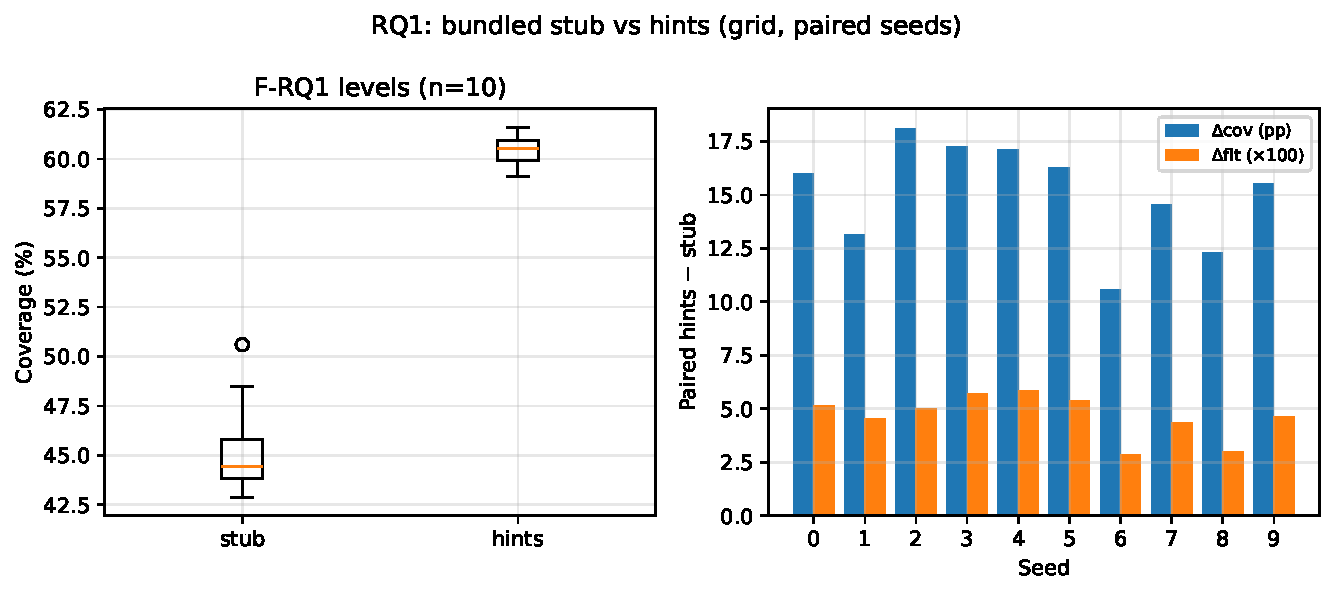
\includegraphics[width=\linewidth]{fig04_rq1_rq0.pdf}
  \caption{Bundled stub vs hints on the primary grid ($n=10$ paired seeds): levels and per-seed paired deltas (stack contrast; see Table~\ref{tab:rq1}).}
  \label{fig:rq1}
\end{figure}

\begin{table}[!htbp]
  \centering
  \caption{Bundled stack: paired hints $-$ stub (grid, $n=10$). $PS$: Eq.~\eqref{eq:ps}. Holm passes as a \emph{stack} outcome; matched H1 is Table~\ref{tab:decomposition}.}
  \label{tab:rq1}
  \fitcenter{%
  \begin{tabular}{@{}lcccccp{2.4cm}@{}}
    \toprule
    Metric & Mean $\Delta$ & Median $\Delta$ & Sign & $PS$ & Wilcoxon $p$ & Causal for H1? \\
    \midrule
    Coverage (pp) & $+15.09 \pm 2.42$ & $+15.20$ & 10/10 & 1.00 & $9.8\times10^{-4}$ & \textbf{No} (confounded) \\
    Mean best fitness & $+0.047 \pm 0.010$ & $+0.046$ & 10/10 & 1.00 & $9.8\times10^{-4}$ & \textbf{No} (confounded) \\
    \bottomrule
  \end{tabular}%
  }
\end{table}

Mean terminal levels: stub $45.32 \pm 2.44$\% coverage, fitness $0.452 \pm 0.041$; hints $60.41 \pm 0.82$\%, fitness $0.499 \pm 0.008$. Bootstrap 95\% CI on median $\Delta$: coverage $[+13.2, +17.1]$~pp; fitness $[+0.038, +0.054]$. Holm $m=2$: both endpoints reject --- the bundled stack passes. Matched-policy H1 follows; per-seed deltas are in Table~\ref{tab:rq1-seeds} (appendix).

\subsection{H1 --- Before-generation surrogate}
\label{sec:decomposition}

\textbf{H1 answer.} At matched \texttt{uniform\_frontier}, live prompt scalars vs.\ stub constants are flat (Table~\ref{tab:decomposition}): mean coverage $60.15 \pm 0.73\%$ vs.\ $60.41 \pm 0.82\%$ ($\Delta = +0.26$~pp; SD~$1.19$~pp; Wilcoxon $p{=}0.41$; bootstrap 95\% CI $[-0.43, +0.98]$~pp). Post-hoc TOST at $|\Delta\mathrm{cov}| \le 2$~pp accepts ($p_{\mathrm{TOST}}{=}6.4\times10^{-4}$; 90\% CI $[-0.43, +0.95]$~pp $\subset [-2,2]$). MDE $\approx 1.2$~pp. Target selection alone recovers $\approx{+}14.8$~pp of the historical $+15$~pp gap (\texttt{stub\_uniform} $-$ \texttt{stub}). Enriched / weak-model pilots ($n{\le}3$; Table~\ref{tab:hint-pilots}) stay within $|\Delta\text{cov}| < 2$~pp. \textbf{Provider scope:} this matched $n{=}10$ TOST is \texttt{qwen-turbo} only; multi-provider Table~\ref{tab:g1} replicates the \emph{bundled} stub-vs-hints contrast (confounded with \texttt{target\_selection}), not matched-policy H1. An exploratory matched-policy pilot on OpenAI \texttt{gpt-4o-mini} (seeds~0--2; \texttt{q1-h1-matched-gpt-4o-mini}) is also flat ($\Delta = -0.47 \pm 0.53$~pp; hints $-$ stub\_uniform). The after-generation surrogate is the separate positive finding (\S\ref{sec:h2}; arm map: appendix Table~\ref{tab:arm-map}).

\begin{table}[!htbp]
  \centering
  \caption{Matched-policy hint channel (H1 only): \texttt{hints} $-$ \texttt{stub\_uniform} on seeds~0--9 ($n{=}10$). Post-hoc TOST/MDE; not a confirmatory Holm set. Single-seed / $n{\le}3$ pilots are in Table~\ref{tab:hint-pilots}.}
  \label{tab:decomposition}
  \small
  \fitcenter{%
  \begin{tabular}{@{}lp{7.2cm}@{}}
    \toprule
    Quantity & Value \\
    \midrule
    Mean coverage (stub\_uniform / hints) & $60.15 \pm 0.73\%$ / $60.41 \pm 0.82\%$ \\
    Mean fitness (stub\_uniform / hints) & $0.496 \pm 0.005$ / $0.499 \pm 0.005$ \\
    Mean $\Delta$cov (hints $-$ stub\_uniform) & $+0.26$~pp (SD~$1.19$~pp) \\
    Bootstrap 95\% CI (mean $\Delta$cov) & $[-0.43, +0.98]$~pp \\
    Wilcoxon (two-sided) & $p{=}0.41$ \\
    TOST $|\Delta\mathrm{cov}|\le 2$~pp (post-hoc) & accept ($p_{\mathrm{TOST}}{=}6.4\times10^{-4}$; 90\% CI $\subset[-2,2]$) \\
    MDE (paired $t$, 80\% power, two-sided) & $\approx 1.2$~pp (power $\approx0.66$ @ 1~pp; $\approx0.997$ @ 2~pp) \\
    \bottomrule
  \end{tabular}%
  }
\end{table}

\begin{table}[!htbp]
  \centering
  \caption{Pilot runs ($n{=}1$ / $n{\le}3$). Enriched / weak-model hint pilots stopped by a pre-set $|\Delta\mathrm{cov}|<2$~pp gate. Not co-tabulated with the matched H1 table (Table~\ref{tab:decomposition}).}
  \label{tab:hint-pilots}
  \small
  \fitcenter{%
  \begin{tabular}{@{}llrp{3.2cm}@{}}
    \toprule
    Arm & Seeds & $\Delta$cov vs.\ \texttt{hints} & Reading \\
    \midrule
    \texttt{hints\_rich} & 0 ($n{=}1$) & $+0.40$~pp & illustrative; underpowered \\
    \texttt{hints\_parent} & 0 ($n{=}1$) & $+0.20$~pp & illustrative; underpowered \\
    \texttt{hints\_direction} & 0 ($n{=}1$) & $-0.68$~pp & illustrative; underpowered \\
    \texttt{hints\_weak} (omni-7b) & 0--2 ($n{=}3$) & $-0.08$~pp vs.\ stub\_uniform & illustrative; underpowered \\
    \texttt{stub\_uniform} (gpt-4o-mini) & 0--2 ($n{=}3$) & $-0.47$~pp vs.\ hints & exploratory; flat \\
    \bottomrule
  \end{tabular}%
  }
  \vspace{0.35em}
  \noindent\small\textit{Note:} $n{=}1$ / $n{\le}3$ pilots; no inferential statistics computed (no $p$-values, no Holm).
\end{table}

\subsection{Non-LLM MAP-Elites baselines (floor + genetic ME)}

\textbf{Bundled floor (passes Holm).} Pure random MAP-Elites (\texttt{vanilla}, 50$\times$ random emitters) reaches $42.36 \pm 0.29$\% coverage and fitness $0.373 \pm 0.005$. Paired hints $-$ vanilla: $\Delta\text{cov} = +18.05 \pm 0.79$~pp (10/10), $\Delta\text{fit} = +0.166 \pm 0.011$ (10/10); Wilcoxon $p = 9.8\times10^{-4}$ for both; Holm $m=2$ rejects; $PS{=}1.00$ on both metrics. This floor contrast mixes emitters and archive policy with the LLM stack.

Descriptive stub $-$ vanilla: $+2.96$~pp coverage.

\textbf{Genetic MAP-Elites.} \texttt{genetic\_me} (20R+30G, default target selection, no LLM) achieves $45.93 \pm 1.50$\%---near historical \texttt{stub} ($45.32 \pm 2.44$\%). Matched-policy \texttt{genetic\_me\_uniform} jumps to $59.04 \pm 0.76$\%; the fair no-LLM reference at matched policy is therefore \texttt{genetic\_me\_uniform} (paired hints $-$ genetic\_me $+14.48$~pp is largely a policy comparison).

\textbf{Performance ladder.} Figure~\ref{fig:ladder} shows mean terminal coverage with 95\% CI on the mean for every arm ($n{=}10$). Ordering: vanilla $<$ stub $\approx$ genetic\_me $\ll$ genetic\_me\_uniform $\approx$ genetic\_me\_filter $\approx$ LLM+\texttt{filter} $\lesssim$ hints $\ll$ cma\_me. The mid-band ($\sim$58--60\%) is where H2 and the LLM stack meet; H2's distinctive claim is coverage \emph{per simulation}, not a higher terminal bar than \texttt{genetic\_me\_uniform} (\S\ref{sec:h2}). Figure~\ref{fig:anytime-ladder} adds evaluation-indexed curves for vanilla / hints / cma\_me ($n{=}5$, median + IQR): CMA-ME leads from early budget (median $\sim$61\% @ 10k vs.\ hints $\sim$47\%).

\begin{figure}[!htbp]
  \centering
  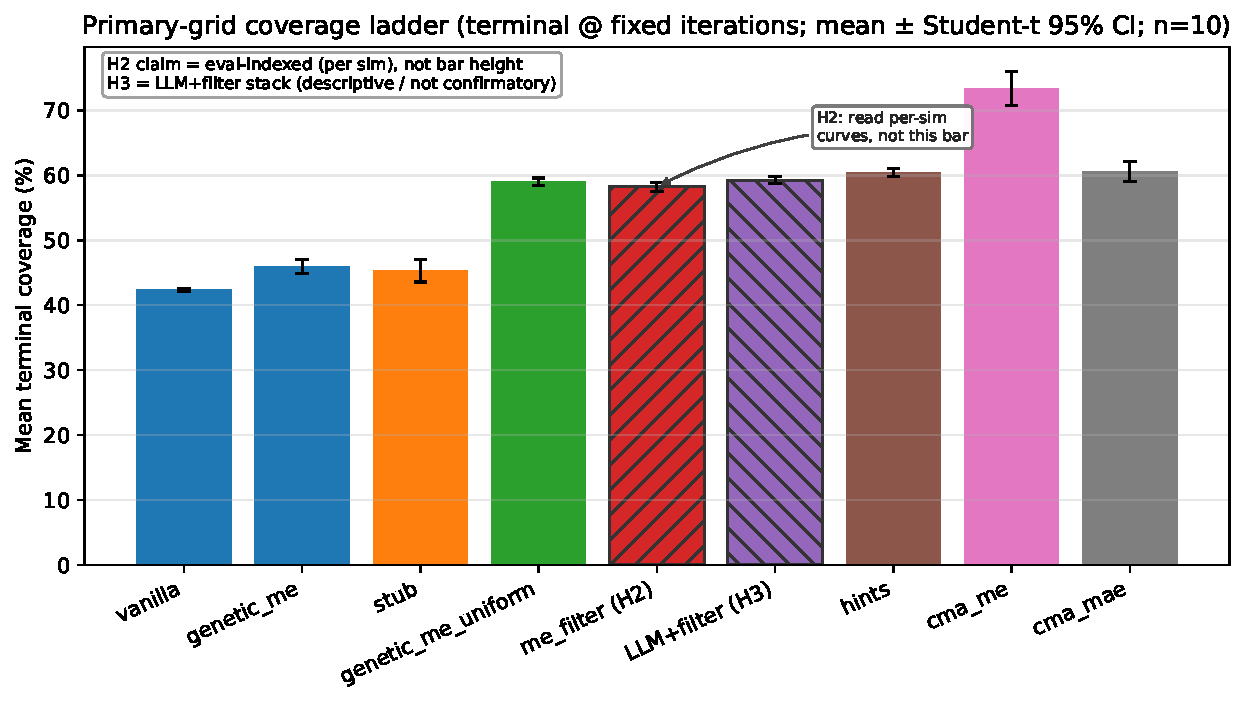
\includegraphics[width=\linewidth]{fig05_ladder.pdf}
  \caption{Mean archive coverage with 95\% CI on the mean for \emph{every} bar ($n{=}10$ paired seeds; normal approx.\ $\bar x \pm 1.96\,s/\sqrt{n}$). Historical \texttt{stub}/\texttt{genetic\_me} use \texttt{min\_fitness\_frontier}; mid-band arms share \texttt{uniform\_frontier}. \texttt{genetic\_me\_filter} and LLM+\texttt{filter} are after-generation (H2) arms.}
  \label{fig:ladder}
\end{figure}

\begin{figure}[!htbp]
  \centering
  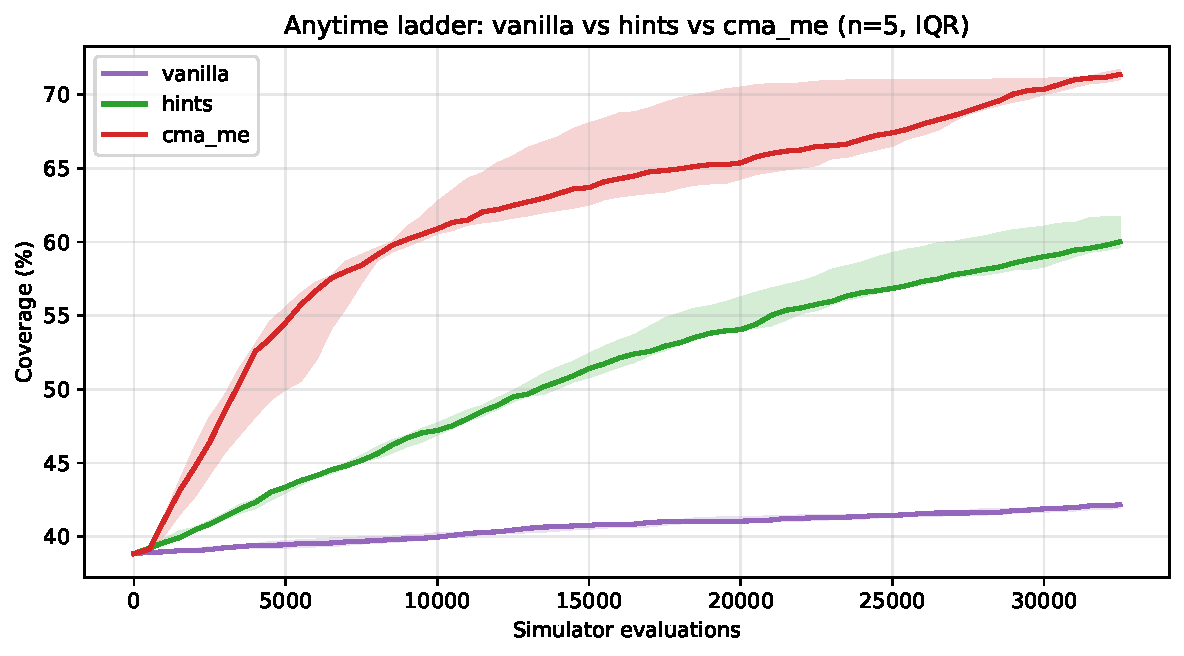
\includegraphics[width=\linewidth]{fig08_anytime_ladder.pdf}
  \caption{Anytime performance ladder: coverage vs.\ simulator evaluations for \texttt{vanilla}, \texttt{hints}, and \texttt{cma\_me} (median + IQR, $n{=}5$ seeds; selective re-runs with \texttt{archive\_trace.jsonl}). CMA-ME separates early ($\sim$+$14$~pp vs.\ hints @ 10k evals); hints and vanilla converge to their terminal bands by 32{,}500 evals.}
  \label{fig:anytime-ladder}
\end{figure}

\subsection{After-generation surrogate (H2)}
\label{sec:h2}

H2 is the only attach role with a measurable evaluation-efficiency gain: matched no-LLM \texttt{genetic\_me\_uniform} vs.\ \texttt{genetic\_me\_filter} (\texttt{uniform\_frontier}, threshold gate, $n=10$; Figure~\ref{fig:acquisition}). This isolates the after-generation surrogate without LLM or before-generation confounds. Do \emph{not} read genetic\_me $46\%$ $\rightarrow$ genetic\_me\_filter $58\%$ as an after-generation effect---that conflates policy with the gate; H2 holds policy fixed at \texttt{uniform\_frontier}.

\begin{figure}[!htbp]
  \centering
  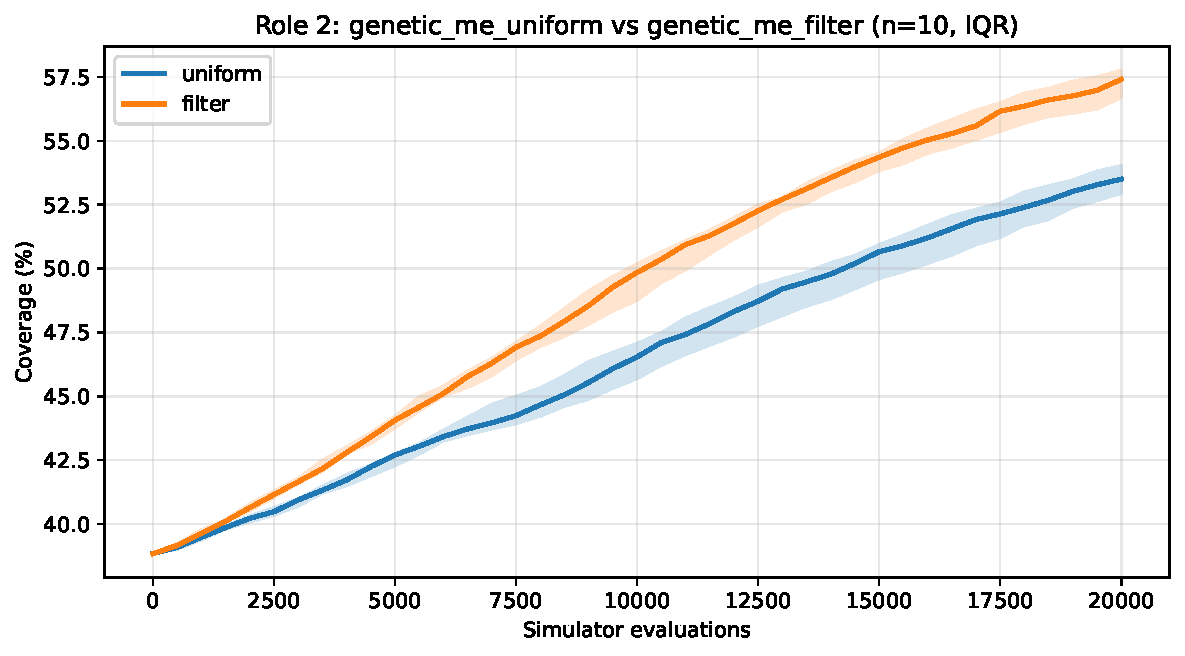
\includegraphics[width=\linewidth]{fig06_acquisition_anytime.pdf}
  \caption{\textbf{Memory figure (eval-efficiency).} Same surrogate, after-generation role only: coverage vs.\ simulator evaluations for \texttt{genetic\_me\_uniform} vs.\ \texttt{genetic\_me\_filter} (median + IQR, $n=10$). Mid-budget gain the before-generation surrogate does \emph{not} deliver at matched policy (\S\ref{sec:decomposition}); not a terminal-coverage or wall-clock win on this evaluator.}
  \label{fig:acquisition}
\end{figure}

We treat \textbf{evaluation-indexed} coverage as the primary H2 axis (Figure~\ref{fig:acquisition})---not terminal coverage or wall clock. At equal evaluation budgets, filter leads by $+3.65$~pp at 20{,}000 evaluations (10/10 seeds) and reaches 50\%/55\% coverage with 28\%/29\% fewer evaluations. At fixed 650 iterations (matched proposal slots, not matched sims), filter uses 33.5\% fewer simulator calls but finishes $-0.83$~pp below uniform ($58.21 \pm 1.03\%$ vs.\ $59.04 \pm 0.76\%$ coverage) and is \emph{slower} in wall time ($\sim$20 vs.\ $\sim$7~min). Of the three practical axes (eval-count, terminal coverage, wall-clock), only the first is positive on this evaluator. Together with matched-policy H1 flat within $\pm 2$~pp at $n{=}10$ (post-hoc TOST), H2 dominates H1 on the evaluation axis alone.

\textbf{Why MLP can cost more than skipped sims.} This is not mysterious invoice noise: acquisition still runs \texttt{predict\_batch} on \emph{every} proposal in the batch (including those later skipped), using a four-member MLP ensemble with MC-dropout uncertainty ($p{=}0.05$) in Python before the cheap simulator roll-out. Simulator evaluations are process-pooled; surrogate inference is a per-candidate Python path whose wall share dominates when $t_{\mathrm{sim}}$ is milliseconds. Skipping 33.5\% of sims therefore removes little wall while adding full-batch MLP work---an engineering trade-off on this domain, not evidence that skip-eval cannot help on expensive simulators.

\textbf{Wall-time break-even (descriptive).} Write wall cost per proposal batch as $(1-s)\,t_{\mathrm{sim}}+t_{\mathrm{MLP}}$ with skip rate $s\approx 0.335$ vs.\ $t_{\mathrm{sim}}$ for full eval. Filter wins on wall only if $t_{\mathrm{MLP}}<s\,t_{\mathrm{sim}}$. Matching the observed wall ratio ($\sim$20 vs.\ $\sim$7~min) implies $t_{\mathrm{MLP}}/t_{\mathrm{sim}}\approx 2.2$ on this evaluator, so the simulator would need to be roughly $\mathbf{7\times}$ slower than today before a 33.5\% skip saves wall clock---an extrapolation to expensive domains, not a measured win on the primary testbed.

\subsection{Why the after-generation surrogate wins (mechanism)}
\label{sec:why-filter}

The H2 gain is not a black box. Logged \texttt{surrogate\_archive.jsonl} rows for \texttt{genetic\_me\_filter} ($n{=}10$; $325{,}000$ proposal slots) show \emph{what} the gate discards (Table~\ref{tab:skip-mech}). Live production filter always recomposed fitness at extinction gate~$0.95$ (scheduler YAML); the compose-gate misalignment discussed in \S\ref{sec:checkpoint} affected only the offline hold-out validity metric, not this live mechanism. All skips cite \texttt{below\_fitness\_threshold} at $\tau{=}0.45$ (skip rate $33.5\%$). Skipped proposals have mean predicted fitness $0.21$ vs.\ $0.61$ for evaluated ones; $81\%$ of skips have predicted early-extinction probability $>0.8$ vs.\ $<0.1\%$ of evaluated proposals; skipped predicted diversity is low (mean $0.24$; $70\%$ with diversity $<0.3$) while evaluated proposals sit in high-diversity bands (mean $0.74$). Uncertainty barely separates the two classes (medians both $\approx 0.16$), so the operative signal is predicted fitness / extinction risk, not calibrated uncertainty. Random emitters contribute disproportionately to skips ($49\%$ of random slots skipped vs.\ $23\%$ of genetic). Among evaluated proposals, only $12.7\%$ realize true fitness $<0.45$ (pred--true MAE $0.066$), consistent with a gate that removes likely dead/low-diversity mass and reallocates the fixed evaluation budget toward niches that can still fill.

This is a mechanistic reading of the after-generation surrogate: it hard-constrains simulator spend. The before-generation surrogate, by contrast, only soft-advises an LLM that already mutates under a JSON grammar; H1's flat matched contrast and no-large-signal enriched pilots are consistent with advice that is easy to ignore.

\textbf{Threshold sensitivity.} A matched-policy sweep (\texttt{q1-h2-threshold-sensitivity}; Table~\ref{tab:h2-tau-sweep}) varies $\tau\in\{0.35,0.45,0.55\}$ at fixed \texttt{uniform\_frontier} ($n{=}10$ each). Skip rate scales monotonically ($24\%$ / $34\%$ / $51\%$). The $\sim$3.7~pp anytime gain at 15--20k evaluations is therefore not an artifact of a single $\tau$: at $\tau{=}0.45$ filter leads 10/10 seeds at both budgets; at $\tau{=}0.35$ mid-budget gain is smaller ($+2.5$~pp @15k, 9/10) but still positive on most seeds; at $\tau{=}0.55$ it is larger at 15k ($+5.4$~pp, 10/10) but terminal coverage falls further ($56.4\%$, paired $\Delta{=}{-}2.6$~pp vs.\ uniform). Aggressive gates trade terminal coverage for faster mid-budget fill; the primary-grid $\tau{=}0.45$ sits in the middle of this trade-off.

\begin{table}[!htbp]
  \centering
  \caption{What the after-generation surrogate skips (\texttt{genetic\_me\_filter}, all seeds; descriptive).}
  \label{tab:skip-mech}
  \small
  \fitcenter{%
  \begin{tabular}{@{}lrr@{}}
    \toprule
    Quantity & Skipped & Evaluated \\
    \midrule
    Share of proposals & $33.5\%$ & $66.5\%$ \\
    Mean predicted fitness & $0.21$ & $0.61$ \\
    Mean pred.\ early-extinction $p$ & $0.90$ & $0.60$ \\
    Share with ext.\ $p>0.8$ & $81\%$ & $<0.1\%$ \\
    Mean predicted diversity & $0.24$ & $0.74$ \\
    Median uncertainty & $0.16$ & $0.16$ \\
    \bottomrule
  \end{tabular}%
  }
\end{table}

\begin{table}[!htbp]
  \centering
  \caption{Threshold sensitivity for \texttt{genetic\_me\_filter} vs.\ matched \texttt{genetic\_me\_uniform} ($n{=}10$ each; descriptive). Anytime $\Delta$ is filter $-$ uniform coverage at matched evaluation budget; terminal $\Delta$ at fixed 650 iterations.}
  \label{tab:h2-tau-sweep}
  \small
  \fitcenter{%
  \begin{tabular}{@{}lrrrrrr@{}}
    \toprule
    $\tau$ & $n$ & Skip & Terminal cov. & $\Delta$ @15k & $\Delta$ @20k & Terminal $\Delta$ \\
    \midrule
    0.35 & 10 & $24.4\%$ & $58.37\%$ & $+2.51$ (9/10) & $+2.67$ (9/10) & $-0.66$ \\
    0.45 & 10 & $33.5\%$ & $58.21\%$ & $+3.72$ (10/10) & $+3.67$ (10/10) & $-0.83$ \\
    0.55 & 10 & $50.7\%$ & $56.41\%$ & $+5.39$ (10/10) & $+2.86$ (10/10) & $-2.62$ \\
    \bottomrule
  \end{tabular}%
  }
\end{table}

\subsection{H3 --- Interaction check (exploratory on locked filter; confirmatory deferred)}
\label{sec:h3}

After H1 (before-generation) and H2 (after-generation), H3 asks whether adding the same after-generation gate to the LLM$+$hint stack helps further. Confirmatory non-inferiority on the **locked production filter** remains blocked ($d{=}0.528 > 0.05$ at $\tau{=}0.45$); we report those levels as exploratory. This version does \emph{not} run new confirmatory seeds; instead we treat the diagnosed mechanism and corrected validity reporting as a standalone Limitations / protocol-amendment contribution (\S\ref{sec:limitations}).

\textbf{Compose-gate mechanism and threshold tuning (offline replay).} The locked $d{=}0.528$ is the production-$\tau$ value, not a $\tau$-invariant constant. Hard fitness recompose zeros the candidate when predicted $p_{\mathrm{ext}}\ge$ extinction gate. During Q1 combat runs, live filter used gate~$0.95$ while hold-out reporting used code default~$0.5$; protocol amendment (2026-07-28) aligns hold-out with runtime (\S\ref{sec:checkpoint}). The compose-gate skip-agreement metric remains the historical live replay comparing skip decisions under gates $0.5$ vs.\ $0.95$ at $\tau{=}0.45$. On logged \texttt{q1-full/filter} proposals ($20$R+$20$G+$10$L; $n{=}10$; $325{,}000$ slots/seed), $74.6\%$ of proposals fall in the ambiguous band $p_{\mathrm{ext}}\in[0.5,0.95)$, where those two gates disagree on whether fitness is zero; outside that band, skip decisions never diverge ($d{=}0$). In-band, about $71\%$ of proposals flip skip/accept at $\tau{=}0.45$ (in-band $d{\approx}0.71$). This localizes blocked H3 to a discontinuous multi-component compose mismatch in the locked combat logs---not to an opaque pipeline failure.

To test whether \texttt{min\_fit} tuning alone removes the block, we replayed the same logs stratified by \texttt{emitter\_type} at $\tau\in\{0.35,0.45,0.55\}$ (artifact: \texttt{filter\_threshold\_emitter\_replay.json}). Skip rates rose monotonically with $\tau$ for every emitter (LLM $16.4\%\!\rightarrow\!32.2\%$; genetic $18.6\%\!\rightarrow\!35.8\%$; random $34.2\%\!\rightarrow\!76.0\%$). Compose-gate divergent-skip fraction $d$ \emph{also} changed with $\tau$ (pooled $0.62\!\rightarrow\!0.53\!\rightarrow\!0.35$; Table~\ref{tab:h3-compose-tau})---$\tau$ and the extinction-gate mismatch interact. At production $\tau{=}0.45$, $d$ remained high and similar across emitters ($0.51$--$0.58$; LLM highest), so emitter-specific $\tau$ calibration in the operating band does not explain away the block. None of the three $\tau$ values brought $d$ below the confirmatory $0.05$ threshold; $d$ falls below $0.05$ only at extreme $\tau$ ($\geq 0.7$, ${>}87\%$ skip)---artifactual gate agreement, not compose repair. We therefore attribute blocked H3 to the historical offline-vs-online extinction-gate mismatch in hard fitness composition on locked combat logs, not to a single mis-set \texttt{min\_fit} knob. Hold-out reporting is now aligned to gate~0.95 (\S\ref{sec:checkpoint}); that fixes the validity headline but does \textbf{not} retroactively pass the locked skip-agreement check or reopen confirmatory H3 without a new pre-specified live criterion. Offline fix-candidate replay on the same logs (\texttt{compose\_gate\_fix\_candidates.json}) confirms that out-of-band proposals have $d{=}0$; force-eval of the gray zone (or skip only when $p_{\mathrm{ext}}\ge 0.95$) drives $d\!\rightarrow\!0$ but cuts skip from $33.5\%$ to $11.7\%$. Soft extinction at $\tau{=}0.45$ over-skips ($96\%$); retargeting soft $\tau$ to $\approx 0.11$ recovers $\sim$32\% skip with only $0.038$ skip-divergence vs.\ hard@$0.95$. Aligning both compose gates to the live $0.95$ setting zeroes $d$ by construction for **new** runs under an amended rule---not for the locked historical replay metric.

\textbf{Deferred confirmatory path (protocol 2026-07-28; not run in this version).} Offline replay motivates \texttt{force\_eval\_extinction\_gray\_zone}: when $p_{\mathrm{ext}}\in[0.5,0.95)$, the filter always evaluates regardless of composed fitness@$\tau{=}0.45$ ($d{=}0$ on replay; skip $\sim$33.5\%$\rightarrow\sim$11.7\%). A deferred H3 repair will compare \texttt{filter\_gray\_zone} to matched \texttt{hints} ($n{=}10$) with the locked non-inferiority margins---deferred to a journal extension. An optional exploratory pilot ($n{=}3$ seeds; same precedent as matched H1 \texttt{gpt-4o-mini} in Table~\ref{tab:hint-pilots}) could sanity-check signal stability before full budget; we did not run it here. Shadow pre-flight for the full matrix targets skip $8$--$18\%$. YAML: \texttt{map\_elites\_scheduler\_nightly\_llm\_filter\_gray\_zone.yaml}. Passing that repair would not retroactively validate historical production \texttt{filter} at 33.5\% skip.

On the bundled LLM tier (locked production \texttt{filter}), \texttt{filter} vs.\ \texttt{hints} is $-1.14$~pp coverage at fixed iterations ($59.27 \pm 0.79\%$ vs.\ $60.41 \pm 0.82\%$). Stacking both slots is not a simple sum of H1$+$H2. Primary after-generation evidence stays H2 (matched genetic arms; \S\ref{sec:h2}). Dungeon and interim maze factorials give the same partial transfer pattern for filter AUC (H2 ports; LLM$+$filter interaction does not; \S\ref{sec:h5}).

\begin{table}[!htbp]
  \centering
  \caption{Offline replay on \texttt{q1-full/filter} ($n{=}10$): skip rate (all emitters) and compose-gate divergent skip $d$ (extinction 0.5 vs.\ 0.95) at each $\tau$.}
  \label{tab:h3-compose-tau}
  \small
  \fitcenter{%
  \begin{tabular}{@{}lrrrrr@{}}
    \toprule
    $\tau$ & Skip (all) & $d$ pooled & $d$ LLM & $d$ genetic & $d$ random \\
    \midrule
    0.35 & $24.4\%$ & $0.619$ & $0.626$ & $0.580$ & $0.654$ \\
    0.45 & $33.5\%$ & $0.528$ & $0.579$ & $0.523$ & $0.508$ \\
    0.55 & $51.2\%$ & $0.351$ & $0.468$ & $0.408$ & $0.236$ \\
    \bottomrule
  \end{tabular}%
  }
\end{table}

\subsection{H4 --- Continuous-relaxation pyribs reference (CMA-ME / CMA-MAE)}
\label{sec:h4}

Pyribs baselines (\texttt{q1-v3-pyribs}, five homogeneous CMA-ES emitters, $n=10$) provide a \textbf{protocol control} under the same warm-start and evaluation budget as other primary-grid arms. Because CMA searches a continuous relaxation with \texttt{rint} decode (\S\ref{sec:pyribs}), this section reports an \textbf{upper-bound-style reference for continuous-friendly representations}---not a validated discrete coverage ceiling against genetic/LLM bit-flip emitters. Mean levels: cma\_me $73.37 \pm 3.65$\%, fitness $0.576 \pm 0.028$; cma\_mae $60.56 \pm 2.16$\%, fitness $0.489 \pm 0.007$; hints $60.41 \pm 0.82$\%, fitness $0.539 \pm 0.008$.

\textbf{Encoding ablation} (\texttt{q1-cma-encoding-ablation}, seeds~0--4, descriptive): alternate rule-bit \emph{decode} and cold-start CMA-ME leave the continuous-relaxation gap intact. These runs vary how continuous proposals map to rule bits; they do \emph{not} test discrete search in the same space as genetic/LLM emitters. \texttt{threshold} ($\geq 0.5$ bits) is \emph{bit-identical} to frozen \texttt{rint} on every seed; \texttt{bernoulli} decode is $-0.46$~pp mean ($72.18\%$); empty-archive \texttt{cold} is $-3.47$~pp ($69.17\%$)---still $\geq +8.8$~pp above hints on every arm mean.

\textbf{Bernoulli-decode CMA-ME (package~C4; \texttt{q1-v3-pyribs-discrete-cma}, $n{=}10$, descriptive).} Same warm-start and 32{,}500-evaluation budget; CMA proposes in $\mathbb{R}^{21}$ but rule bits are Bernoulli-sampled at decode (discrete genotypes at evaluation, continuous covariance adaptation unchanged). Mean coverage $71.25 \pm 2.88$\%, fitness $0.578 \pm 0.020$. Paired vs.\ \texttt{hints}: $+10.84 \pm 2.94$~pp (10/10 seeds); vs.\ \texttt{genetic\_me\_uniform}: $+12.22 \pm 2.56$~pp (10/10); vs.\ \texttt{rint} CMA-ME: $-2.12 \pm 4.93$~pp (3/10).

\textbf{Native discrete-search CMA-ME (\texttt{q1-v3-pyribs-native-discrete-cma}, $n{=}10$, descriptive).} Custom \texttt{DiscreteCMAEmitter}: bit-flip on rule bits + Gaussian on floats, discrete $\{0,1\}$ genotype stored in archive, $\sigma$ adapted by a 1/5 success rule (MVP). Mean coverage $65.57 \pm 3.40$\%, fitness $0.542 \pm 0.028$. Paired vs.\ \texttt{hints}: $+5.16 \pm 3.67$~pp (10/10); vs.\ \texttt{genetic\_me\_uniform}: $+6.54 \pm 3.76$~pp (10/10); vs.\ Bernoulli: $-5.68 \pm 5.90$~pp (1/10); vs.\ \texttt{rint}: $-7.80 \pm 5.07$~pp (0/10).

\textbf{pbCMA CMA-ME (\texttt{q1-v3-pyribs-pbcma}, $n{=}10$, descriptive).} \texttt{PBCMAEmitter}: latent $(\mu/\mu_w,\lambda)$-CMA on $\mathbb{R}^{21}$ with bit threshold at $0.5$, margin correction, and CMA updates from \emph{latent} ranked parents (discrete $\{0,1\}$ genotype stored in archive). Mean coverage $69.95 \pm 5.42$\%, fitness $0.548 \pm 0.034$. Paired vs.\ \texttt{hints}: $+9.54 \pm 5.25$~pp (10/10); vs.\ \texttt{genetic\_me\_uniform}: $+10.92 \pm 5.80$~pp (10/10); vs.\ native bit-flip: $+4.38 \pm 5.93$~pp (8/10); vs.\ Bernoulli: $-1.30 \pm 6.54$~pp (4/10); vs.\ \texttt{rint}: $-3.42 \pm 7.12$~pp (2/10). Latent covariance adaptation therefore recovers most of the MVP bit-flip deficit vs.\ Bernoulli and nearly half the \texttt{rint} gap, but continuous-relaxation \texttt{rint} still leads on eight seeds---consistent with a modest residual encoding advantage, not ``any CMA-ME pipeline wins.''

Paired hints $-$ cma\_me: $\Delta\text{cov} = -12.96 \pm 3.46$~pp (0/10 positive), $\Delta\text{fit} = -0.077 \pm 0.029$ (0/10); CMA-ME dominates coverage on every seed (largest gap at seed~4: $-20.0$~pp). Paired hints $-$ cma\_mae: $\Delta\text{cov} = -0.15 \pm 2.25$~pp (5/10), $\Delta\text{fit} = +0.010 \pm 0.008$ (10/10) --- near parity on coverage, with a small mean-fitness edge for hints.

\begin{figure}[!htbp]
  \centering
  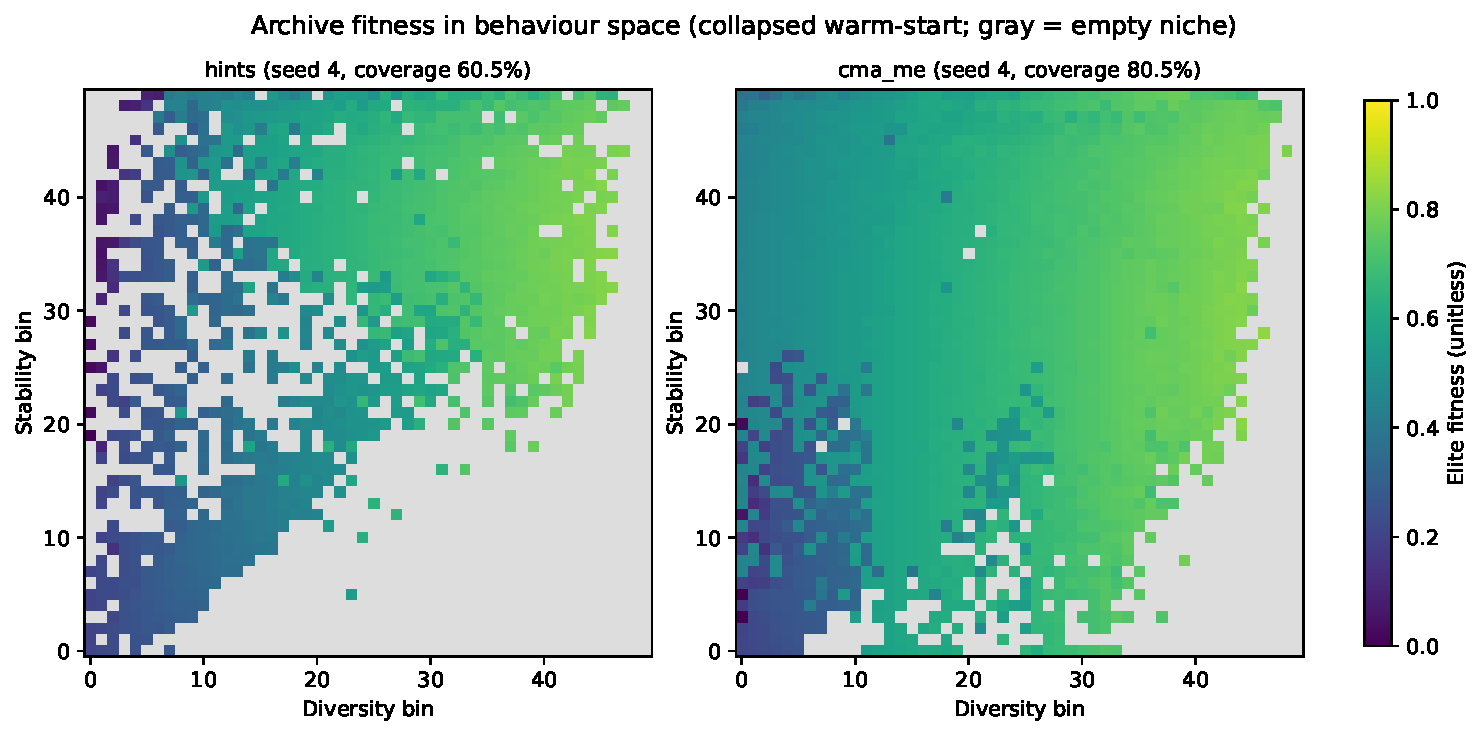
\includegraphics[width=\linewidth]{fig07_archive_heatmaps_seed4.pdf}
  \caption{Archive fitness in stability--diversity space: paired seed~4, LLM+scalar hints vs.\ CMA-ME (collapsed warm-start archives). Gray = empty niches; shared colour scale $[0,1]$. Coverage: hints 60.5\%, cma\_me 80.5\%. CMA-ME fills large low-diversity and mid-archive holes that remain empty under hints. Supplemental paired seeds with smaller/mid gaps (seeds~1, 6; $\Delta$cov $-9.4$ / $-16.0$~pp) and the three-seed panel: appendix Figure~\ref{fig:heatmap-panel}.}
  \label{fig:heatmaps}
\end{figure}

Figure~\ref{fig:heatmaps} shows where the $\approx$13--20~pp coverage gap lives on a representative seed: CMA-ME illuminates broad regions of behaviour space that hints leave empty---especially low-diversity bands and scattered interior holes---rather than only polishing already-filled high-fitness niches. Fitness colour is higher on average in the CMA panel, consistent with the fitness delta, but the dominant visual story is \emph{coverage}: gradient variation reaches niches the heterogeneous LLM stack does not. The gap is also visible along the evaluation axis (Figure~\ref{fig:anytime-ladder}): on seed~4, CMA-ME reaches $\sim$63\% coverage by 10{,}000 evaluations while hints are still $\sim$47\%.

\textbf{H4 outcome (does not pass).} Holm $m=4$ (Table~\ref{tab:frq-ceiling}): hints do not beat \emph{both} pyribs arms simultaneously (only the CMA-MAE fitness contrast rejects). Under continuous-relaxation encoding, CMA-ME leads hints by $\sim$13~pp on coverage. We report this as an upper-bound reference, \emph{not} as a discrete emitter ranking: Bernoulli-decode ($+10.8$~pp vs.\ hints), pbCMA ($+9.5$~pp), and native bit-flip ($+5.2$~pp) all lead hints, but only pbCMA/Bernoulli approach \texttt{rint} on mean coverage and neither matches \texttt{rint} seed-wise (pbCMA 2/10; Bernoulli 3/10).

\begin{table}[!htbp]
  \centering
  \caption{Pyribs continuous-relaxation reference (H4): Holm step-down ($m=4$, paired hints $-$ arm, one-sided greater). Not an H2 contrast; repository analysis ID in Table~\ref{tab:families}. $PS$: Eq.~\eqref{eq:ps}.}
  \label{tab:frq-ceiling}
  \small
  \fitcenter{%
  \begin{tabular}{@{}llrrcc@{}}
    \toprule
    Test & Arm / metric & Mean $\Delta$ & Raw $p$ & $PS$ & Holm reject \\
    \midrule
    H4\_mae\_fit & cma\_mae fitness & $+0.010$ & $9.8\times10^{-4}$ & 1.00 & \textbf{Yes} \\
    H4\_mae\_cov & cma\_mae coverage & $-0.15$~pp & 0.50 & 0.50 & No \\
    H4\_me\_cov & cma\_me coverage & $-12.96$~pp & 1.0 & 0.00 & No \\
    H4\_me\_fit & cma\_me fitness & $-0.077$ & 1.0 & 0.00 & No \\
    \bottomrule
  \end{tabular}%
  }
\end{table}

\subsection{Multi-LLM replication}

We replicated the bundled LLM+constants vs.\ LLM+scalars contrast on two additional providers with identical schedulers (6{,}500 LLM calls per run). Table~\ref{tab:g1} reports each provider separately---never pooled. Both additional providers pass the per-provider bundled contrast at $n{=}10$ (Holm $m{=}2$ on conjunctive $\Delta$cov+$\Delta$fit; both reject per provider). \textbf{This is not matched H1:} G1 keeps the historical stub arm (\texttt{min\_fitness\_frontier}), so provider replication supports the confounded stack $\Delta$, not the matched-policy \texttt{stub\_uniform}-vs-\texttt{hints} null.

\begin{table}[!htbp]
  \centering
  \caption{Multi-provider: \emph{bundled} hints $-$ stub \emph{by} LLM provider (confounded with \texttt{target\_selection}). Not matched-policy H1. \textbf{Not to be read as a combined effect:} rows are separate experiments (never pool or average $\Delta$ across LLMs); Holm applies per provider at matched $n$.}
  \label{tab:g1}
  \fitcenter{%
  \begin{tabular}{@{}lcccl@{}}
    \toprule
    Provider & $\Delta$cov (pp) & $\Delta$fit & Sign (cov) & Outcome \\
    \midrule
    qwen-turbo (v2 reference, $n{=}10$) & $+15.09$ & $+0.053$ & 10/10 & passes \\
    DeepSeek V4 Pro ($n{=}10$) & $+16.95 \pm 2.12$ & $+0.052 \pm 0.013$ & 10/10 & passes \\
    OpenAI gpt-4o-mini ($n{=}10$) & $+9.66 \pm 2.41$ & $+0.018 \pm 0.013$ & 10/10 & passes \\
    \bottomrule
  \end{tabular}%
  }
\end{table}

DeepSeek matches the qwen-turbo reference in magnitude and absolute hint-arm coverage ($\sim$62\% vs.\ $\sim$60\%). gpt-4o-mini replicates direction at full power ($p_{\mathrm{cov}}{=}0.001$, $p_{\mathrm{fit}}{=}0.003$ at $n{=}10$) but absolute hint-arm coverage is lower ($55.3\%$); stub arms align across providers ($\sim$45\% coverage), suggesting cross-model gaps concentrate in LLM-driven variation under hints. Because levels differ by API, averaging the three $\Delta$cov rows would be methodologically wrong.

\subsection{Cost and wall time (descriptive)}
\label{sec:cost}

Matched \emph{evaluation} budget (32{,}500 sims) is \emph{not} matched dollar or wall cost (Table~\ref{tab:cost}). Mixed LLM arms issue 6{,}500 chat completions per seed ($\sim$90\% of wall is HTTP emit time). Using published international DashScope \texttt{qwen-turbo} list rates ($\approx$\$0.05/M input, \$0.20/M output tokens; mid-2026) and a conservative $\sim$1.5k~in~/~0.25k~out tokens per emit, API spend is on the order of \textbf{$\sim\$1$--2 per seed} for \texttt{hints}/\texttt{stub}/\texttt{filter} ($\sim\$10$--20 for $n{=}10$); genetic and pyribs arms have \$0 API. Exact invoices vary with prompt length and region; we report call counts as the primary opaque budget and dollars as an order-of-magnitude guide.

On this cheap evaluator, the after-generation surrogate \emph{increases} wall time despite fewer simulations (break-even in \S\ref{sec:results}). Dungeon LLM arms require $\sim$51--57~min at 5k proposals vs.\ $<$1~min for genetic ME.

\textbf{Matched-dollar reading.} At near-equal coverage, \texttt{genetic\_me\_uniform} ($59.0\%$, $\sim$6~min, \$0 API) is Pareto-superior to \texttt{hints} ($60.4\%$, $\sim$94~min, $\sim$6.5k LLM calls / $\sim\$1$--2) on wall and money for a $\approx{+}1.4$~pp coverage gap. Under continuous-relaxation encoding, CMA-ME reaches higher terminal coverage at moderate wall and \$0 API (\S\ref{sec:h4}); among \emph{discrete} emitters at matched policy, \texttt{genetic\_me\_uniform} dominates \texttt{hints} on wall/API. Matched-eval contrasts should not be read as matched-cost competitiveness of the LLM stack.

\begin{table}[!htbp]
  \centering
  \caption{Mean cost per seed on the primary grid tier ($n=10$; descriptive). Wall from run summaries; LLM calls from \texttt{llm\_emit\_attempts}; API \$ is an order-of-magnitude estimate at published \texttt{qwen-turbo} intl.\ rates (see text), not an invoice.}
  \label{tab:cost}
  \small
  \fitcenter{%
  \begin{tabular}{@{}lrrr@{}}
    \toprule
    Condition & Wall (min) & LLM calls & Est.\ API (\$) \\
    \midrule
    \texttt{vanilla} & $4.4$ & 0 & 0 \\
    \texttt{genetic\_me\_uniform} & $6.3$ & 0 & 0 \\
    \texttt{genetic\_me\_filter} & $19.9$ & 0 & 0 \\
    \texttt{cma\_me} & $22.3$ & 0 & 0 \\
    \texttt{cma\_mae} & $23.4$ & 0 & 0 \\
    \texttt{stub} & $70.4$ & 6{,}500 & $\sim$1--2 \\
    \texttt{hints} & $93.6$ & 6{,}500 & $\sim$1--2 \\
    \texttt{filter} & $108.5$ & 6{,}500 & $\sim$1--2 \\
    \bottomrule
  \end{tabular}%
  }
\end{table}

\subsection{H5 --- Cross-domain after-generation check (dungeon + maze; not cross-domain LLM QD)}
\label{sec:h5}

\textbf{Scope of this subsection.} We ask whether the after-generation surrogate \emph{ports} beyond the primary evaluator, not whether the bundled LLM+surrogate stack generalizes. The locked confirmatory check is a 16$\times$16 patch-LLM dungeon under frozen v4 (\texttt{q1-v4-dungeon-rerun}, $n{=}10$, 5{,}000 proposals/arm). A journal-track maze factorial at the primary-grid proposal budget (\texttt{q1-v5-maze-full}, 32{,}500 proposals/arm) is reported as an interim third-domain slice below. Neither is a claim of cross-domain LLM QD superiority. Timing-to-coverage thresholds from the first dungeon pilot remain exploratory; confirmatory endpoints are AUC at matched real evaluations. Dungeon quality gates passed (LLM fallback $\le 0.99\%$, filter skip 34--40\%). Figure~\ref{fig:b4} shows dungeon anytime curves. A supplementary dungeon CPU after-generation pair at 32{,}500 proposals is reported in Table~\ref{tab:b4-fullcpu}; full-budget LLM dungeon arms remain deferred.

\paragraph{Dungeon (locked H5).}
A 16$\times$16 patch-LLM dungeon under frozen v4 asks the transfer question on a confirmatory AUC family (appendix Table~\ref{tab:families}).

\begin{figure}[!htbp]
  \centering
  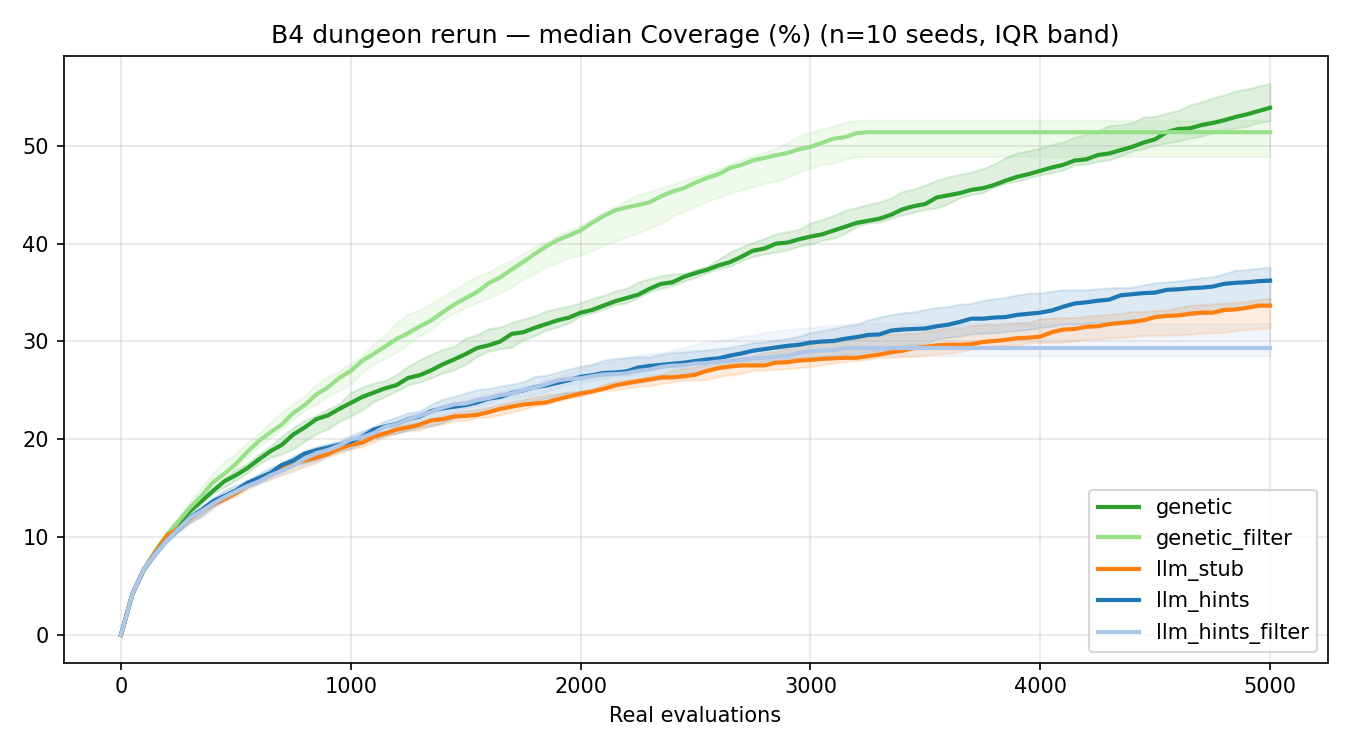
\includegraphics[width=0.48\linewidth]{fig_b4_anytime_coverage.png}
  \hfill
  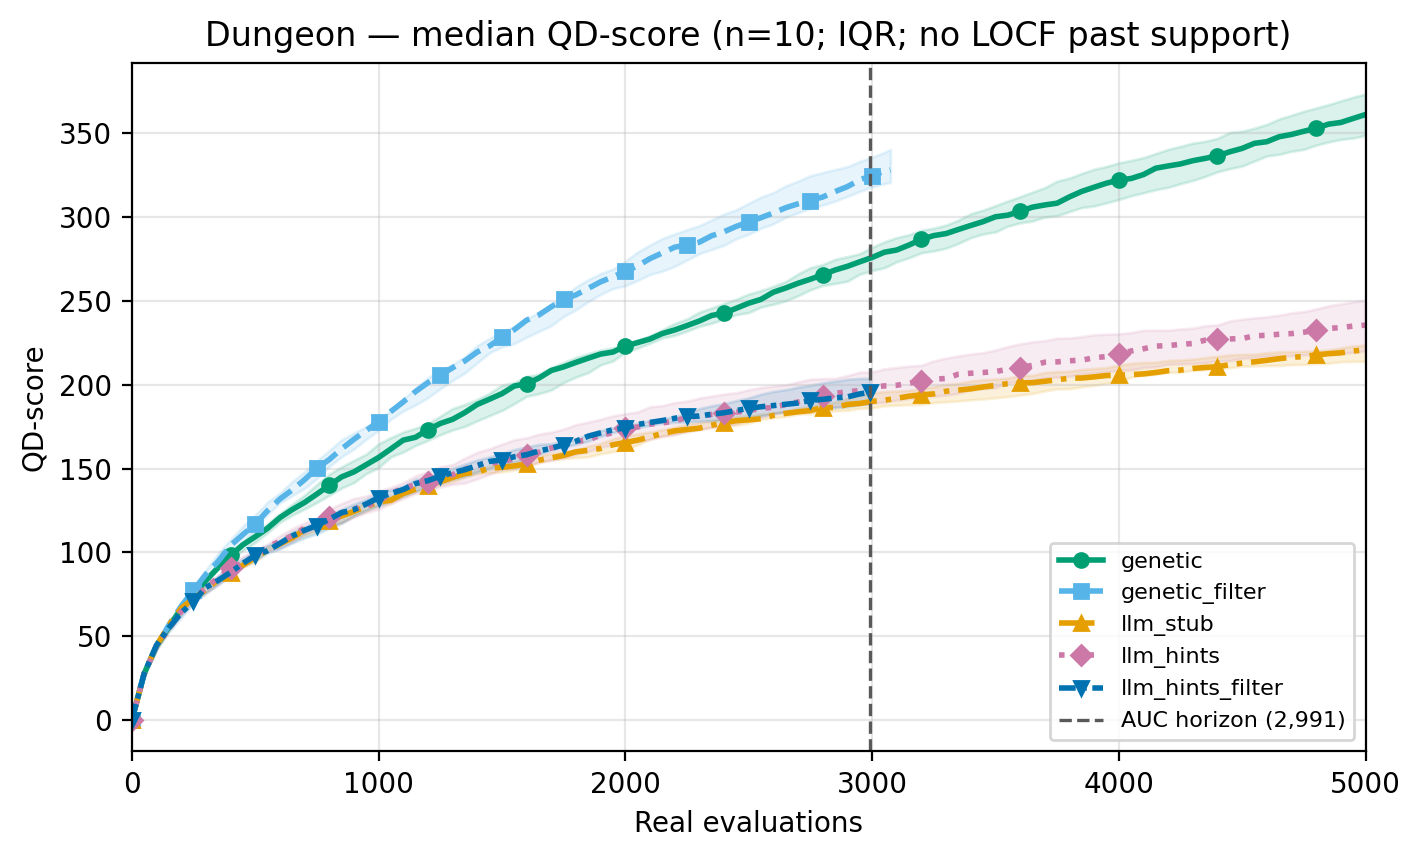
\includegraphics[width=0.48\linewidth]{fig_b4_anytime_qd_score.png}
  \caption{Dungeon domain anytime curves (5k proposals/arm, $n=10$ seeds): coverage (left) and QD-score (right).}
  \label{fig:b4}
\end{figure}

At fixed proposals (Table~\ref{tab:b4}): local genetic MAP-Elites dominates all LLM arms ($54.82 \pm 3.11$\% vs.\ llm\_hints $35.60 \pm 2.21$\%; $+19.2$~pp, 10/10). Mean elite fitness is flat ($\sim$0.73--0.74); gains are coverage-driven. Descriptive hints $-$ stub: $+2.31$~pp (9/10). Filter arms finish lower at fixed proposals (genetic\_filter $-4.4$~pp; llm\_hints\_filter $-5.4$~pp vs.\ unfiltered).

\begin{table}[!htbp]
  \centering
  \caption{Dungeon mean levels at 5{,}000 proposals ($n=10$).}
  \label{tab:b4}
  \fitcenter{%
  \begin{tabular}{@{}lrrrr@{}}
    \toprule
    Arm & Coverage (\%) & Mean fit & QD-score & Skip (\%) \\
    \midrule
    genetic & $54.82 \pm 3.11$ & 0.738 & 364 & 0 \\
    genetic\_filter & $50.39 \pm 3.13$ & 0.739 & 335 & 36.5 \\
    llm\_stub & $33.29 \pm 1.97$ & 0.734 & 220 & 0 \\
    llm\_hints & $35.60 \pm 2.21$ & 0.735 & 235 & 0 \\
    llm\_hints\_filter & $30.22 \pm 2.25$ & 0.735 & 200 & 37.1 \\
    \bottomrule
  \end{tabular}%
  }
\end{table}

At a matched real-evaluation checkpoint (2{,}991 evals), genetic\_filter beats genetic by $+7.83$~pp (10/10); hints beats stub by $+1.52$~pp (8/10). Locked dungeon H5 is \textbf{partial} (Holm $m=8$, AUC at matched budget; Table~\ref{tab:b4-holm}): genetic\_filter $-$ genetic coverage and QD-score AUC pass (H2 ports); hints $-$ stub and LLM+filter interaction do not survive correction. \textbf{Readout:} the after-generation surrogate without LLM transfers; bundled LLM QD lift and ``hints beat stub'' do \emph{not}. Genetic MAP-Elites remains the strong dungeon baseline ($\sim$19~pp above LLM hints at fixed proposals).

\textbf{Supplementary CPU @ 32{,}500 proposals} (\texttt{q1-v4-dungeon-full-cpu}, $n{=}10$; not part of the locked dungeon H5 AUC set). At fixed proposal slots both arms saturate ($89.42 \pm 0.77$\% genetic vs.\ $88.79 \pm 1.75$\% genetic\_filter; $-0.63$~pp), while filter skips $30.8\%$ of slots ($\sim$22.5k real evals vs.\ 32.5k). On the evaluation axis, filter AUC still leads at matched budget (22{,}155 evals; Table~\ref{tab:b4-fullcpu}): coverage AUC $+3.6$~pp (9/10; Holm reject) and QD-score AUC $+33.9$ (8/10; Holm reject). This mirrors the primary after-generation pattern: sample-efficiency on evals, not a free terminal win at fixed proposal count.

\textbf{Dungeon filter mechanism (descriptive).} The dungeon gate uses $\tau{=}0.78$ (separate checkpoint calibration), not the primary-grid $\tau{=}0.45$. Skip logs on \texttt{genetic\_filter} ($325{,}000$ proposal slots @ 32.5k) discard low predicted fitness at low uncertainty (mean pred.\ fitness $0.71$ skipped vs.\ $0.63$ evaluated; mean uncertainty $0.03$ vs.\ $0.08$); all skips cite \texttt{below\_fitness\_threshold}. Empty bins are still explored ($\lesssim$2\% of evaluated rows @ 5k).

\begin{table}[!htbp]
  \centering
  \caption{Supplementary dungeon after-generation surrogate @ 32{,}500 proposals (\texttt{q1-v4-dungeon-full-cpu}, $n{=}10$).}
  \label{tab:b4-fullcpu}
  \small
  \fitcenter{%
  \begin{tabular}{@{}lrrrr@{}}
    \toprule
    Arm & Coverage (\%) & Mean evals & Skip (\%) & AUC contrast \\
    \midrule
    genetic & $89.42 \pm 0.77$ & 32{,}500 & 0 & --- \\
    genetic\_filter & $88.79 \pm 1.75$ & 22{,}480 & 30.8 & filter $-$ genetic \\
    \midrule
    \multicolumn{5}{@{}l@{}}{Coverage AUC @ 22{,}155 matched evals: $+3.6$~pp mean (9/10; Holm reject)} \\
    \multicolumn{5}{@{}l@{}}{QD-score AUC @ 22{,}155 matched evals: $+33.9$ mean (8/10; Holm reject)} \\
    \bottomrule
  \end{tabular}%
  }
\end{table}

\begin{table}[!htbp]
  \centering
  \caption{Dungeon Holm outcomes ($m{=}8$; AUC @ 2{,}991 real evaluations, $n=10$). All eight family tests are listed; only the two genetic\_filter contrasts reject after Holm.}
  \label{tab:b4-holm}
  \small
  \fitcenter{%
  \begin{tabular}{@{}lrrc@{}}
    \toprule
    Contrast (AUC) & Mean $\Delta$ & Raw $p$ & Holm reject \\
    \midrule
    genetic\_filter $-$ genetic (coverage) & $+0.048$ & $9.8\times10^{-4}$ & \textbf{Yes} \\
    genetic\_filter $-$ genetic (QD-score) & $+29.9$ & $9.8\times10^{-4}$ & \textbf{Yes} \\
    hints $-$ stub (coverage) & $+0.008$ & 0.032 & No \\
    hints $-$ stub (QD-score) & $+5.3$ & 0.019 & No \\
    llm\_hints\_filter $-$ llm\_hints (coverage) & $\approx 0$ & 0.50 & No \\
    llm\_hints\_filter $-$ llm\_hints (QD-score) & $-0.77$ & 0.69 & No \\
    acquisition interaction (coverage) & $-0.048$ & 1.0 & No \\
    acquisition interaction (QD-score) & $-30.7$ & 1.0 & No \\
    \bottomrule
  \end{tabular}%
  }
\end{table}

\paragraph{Maze (journal-track H5; interim $n{=}5$).}
\label{sec:h5-maze}
A maze factorial mirrors the dungeon five-arm design at the primary-grid proposal budget (\texttt{q1-v5-maze-full}; 32{,}500 proposals/arm; 900-cell grid; maze filter $\tau{=}0.685$). We report seeds $0$--$4$ as an interim five-arm slice; genetic vs.\ genetic\_filter is already complete for seeds $0$--$9$. Quality gates pass on the interim slice (pooled LLM fallback $0.016\%$; genetic\_filter skip $27.4 \pm 0.6\%$; parse success $\ge 99.89\%$).

At fixed proposals (Table~\ref{tab:b5}): genetic arms saturate the 900-cell archive ($99.2 \pm 1.7$\% genetic; $99.3 \pm 1.6$\% genetic\_filter), while LLM arms plateau near half coverage (llm\_hints $46.6 \pm 3.1$\%; llm\_stub $47.1 \pm 4.5$\%; llm\_hints\_filter $43.4 \pm 4.8$\%). The terminal genetic$-$LLM gap ($\sim$52~pp) is therefore a \textbf{ceiling artifact} on the genetic side (saturation by $\sim$14k evaluations) plus a real emitter gap---not a fair terminal-coverage ranking. Descriptive hints$-$stub is near zero at the terminal ($-0.5$~pp); llm\_hints\_filter finishes $-3.2$~pp vs.\ hints.

\begin{table}[!htbp]
  \centering
  \caption{Maze mean levels at 32{,}500 proposals (interim seeds $0$--$4$, $n{=}5$). Genetic arms hit a 900-cell ceiling; primary endpoints are AUC at matched evaluations (Table~\ref{tab:b5-holm}).}
  \label{tab:b5}
  \fitcenter{%
  \begin{tabular}{@{}lrrrr@{}}
    \toprule
    Arm & Coverage (\%) & QD-score & Skip (\%) & Wall (min) \\
    \midrule
    genetic & $99.2 \pm 1.7$ & 573 & 0 & $\sim$0.8 \\
    genetic\_filter & $99.3 \pm 1.6$ & 573 & 27.4 & $\sim$1.1 \\
    llm\_stub & $47.1 \pm 4.5$ & 248 & 0 & $\sim$393 \\
    llm\_hints & $46.6 \pm 3.1$ & 245 & 0 & $\sim$342 \\
    llm\_hints\_filter & $43.4 \pm 4.8$ & 229 & 28.2 & $\sim$355 \\
    \bottomrule
  \end{tabular}%
  }
\end{table}

At matched real evaluations (22{,}860 evals; Table~\ref{tab:b5-holm}), genetic\_filter leads genetic on coverage AUC by $+4.7$~pp (5/5; raw $p{=}0.031$) and on QD-score AUC by $+32.2$ (5/5). Hints$-$stub coverage AUC is $+1.9$~pp (4/5; raw $p{=}0.094$). LLM$+$filter and acquisition interaction are negative (1/5 and 0/5). Interim five-arm Holm $m{=}8$ does \textbf{not} pass: no contrast survives correction at $n{=}5$ (underpowered vs.\ dungeon $n{=}10$). The pattern nevertheless matches locked dungeon H5: H2-direction consistent; hints and LLM$+$filter do not.

\textbf{Supplementary maze CPU @ 32{,}500 proposals} (genetic vs.\ genetic\_filter only, seeds $0$--$9$; Table~\ref{tab:b5-fullcpu}). Terminal coverage is again saturated ($\sim$99.6\% both arms; skip $27.3\%$). On the evaluation axis at 23{,}300 matched evals, filter AUC rejects after Holm: coverage $+4.6$~pp (10/10) and QD-score $+30.2$ (10/10). This is the third domain (primary grid $\rightarrow$ dungeon $\rightarrow$ maze) on which after-generation sample-efficiency ports without an LLM.

\begin{table}[!htbp]
  \centering
  \caption{Supplementary maze after-generation surrogate @ 32{,}500 proposals (genetic vs.\ genetic\_filter, $n{=}10$).}
  \label{tab:b5-fullcpu}
  \small
  \fitcenter{%
  \begin{tabular}{@{}lrrrr@{}}
    \toprule
    Arm & Coverage (\%) & Mean evals & Skip (\%) & AUC contrast \\
    \midrule
    genetic & $99.62 \pm 1.19$ & 32{,}500 & 0 & --- \\
    genetic\_filter & $99.64 \pm 1.12$ & 23{,}614 & 27.3 & filter $-$ genetic \\
    \midrule
    \multicolumn{5}{@{}l@{}}{Coverage AUC @ 23{,}300 matched evals: $+4.6$~pp mean (10/10; Holm reject)} \\
    \multicolumn{5}{@{}l@{}}{QD-score AUC @ 23{,}300 matched evals: $+30.2$ mean (10/10; Holm reject)} \\
    \bottomrule
  \end{tabular}%
  }
\end{table}

\begin{table}[!htbp]
  \centering
  \caption{Maze Holm outcomes (interim H5; $m{=}8$; AUC @ 22{,}860 real evaluations, seeds $0$--$4$). No contrast survives Holm at $n{=}5$; genetic\_filter signs are 5/5. Replace with $n{=}10$ when seeds 5--9 LLM arms complete.}
  \label{tab:b5-holm}
  \small
  \fitcenter{%
  \begin{tabular}{@{}lrrc@{}}
    \toprule
    Contrast (AUC) & Mean $\Delta$ & Raw $p$ & Holm reject \\
    \midrule
    genetic\_filter $-$ genetic (coverage) & $+0.047$ & 0.031 & No \\
    genetic\_filter $-$ genetic (QD-score) & $+32.2$ & 0.031 & No \\
    hints $-$ stub (coverage) & $+0.019$ & 0.094 & No \\
    hints $-$ stub (QD-score) & $+11.3$ & 0.063 & No \\
    llm\_hints\_filter $-$ llm\_hints (coverage) & $-0.017$ & 0.938 & No \\
    llm\_hints\_filter $-$ llm\_hints (QD-score) & $-8.6$ & 0.938 & No \\
    acquisition interaction (coverage) & $-0.063$ & 1.0 & No \\
    acquisition interaction (QD-score) & $-40.8$ & 1.0 & No \\
    \bottomrule
  \end{tabular}%
  }
\end{table}

\textbf{H5 readout (dungeon + interim maze).} After-generation sample-efficiency without LLM transfers on both secondary domains (dungeon H2 AUC passes Holm; maze CPU $n{=}10$ H2 AUC passes Holm; maze five-arm interim 5/5 signs, underpowered). Bundled LLM QD lift does \emph{not} transfer: genetic MAP-Elites leads LLM arms by $\sim$19~pp on dungeon and $\sim$40~pp on maze coverage AUC at matched evals. Hints vs.\ stub remains a small descriptive AUC edge that does not survive Holm. LLM$+$filter interaction stays negative.

\section{Discussion}
\label{sec:discussion}

\subsection{Synthesis}

These observations suggest that, for LLM-guided QD, \emph{where} a surrogate attaches can matter more than which pipeline wins a bake-off (Figure~\ref{fig:pipeline}). Under one shared MLP checkpoint on this evaluator, the after-generation surrogate (H2; Figure~\ref{fig:acquisition}) improves coverage per simulation, while the matched-policy before-generation surrogate (H1) stays within $\pm 2$~pp at $n{=}10$ (post-hoc TOST). That asymmetry is the intended payoff of attachment-point decomposition: the after-generation surrogate hard-gates evaluation spend (SAIL-\emph{kin}), whereas the before-generation surrogate supplies prompt-side advice that never skips \texttt{evaluate\_candidate}. H3 levels further suggest that stacking both under LLM is not a simple sum; confirmatory interaction testing is deferred (dual compose gate diagnosed; gray-zone repair; \S\ref{sec:h3}, \S\ref{sec:limitations}). Magnitudes are testbed-specific; the before/after framing is intended as a reusable question for LLM-guided QD stacks, not a universal ranking.

\subsection{Mechanistic reading}
\label{sec:why-discussion}

Results report \emph{what} moved (Fig.~\ref{fig:acquisition}); the skip logs and matched contrasts suggest a candidate \emph{why}.

\begin{itemize}
  \item \textbf{Budget reallocation.}
 These observations suggest that the after-generation surrogate mainly reallocates simulator spend rather than inventing stronger proposals. Skip logs (\S\ref{sec:why-filter}) show discarded proposals concentrated at low predicted fitness (mean $0.21$ vs.\ $0.61$ evaluated), high extinction risk ($81\%$ of skips with $p>0.8$), and low diversity, while uncertainty barely separates skip from evaluate. At matched evaluations that discarded mass frees slots for niches that can still fill ($+3.65$~pp @ 20k); at fixed iterations the same gate finishes $-0.83$~pp---a pattern consistent with reallocation under a fixed proposal schedule.
  \item \textbf{Shared checkpoint, asymmetric use.}
 Offline hold-out at runtime-aligned gate~$0.95$ gives $R^2_{\mathrm{fitness}}{=}0.94$ with NMAE$=0.112$ (\S\ref{sec:checkpoint})---scale-normalized absolute error is \emph{worse} than the historical gate-$0.5$ NMAE$=0.052$, so the checkpoint is less accurate in absolute units than the original $R^2{=}0.76$ headline suggested.
 The relevant claim for H2 is weaker and mechanistic: live skip logs (always composed at gate~$0.95$; Table~\ref{tab:skip-mech}) still separate skip vs.\ evaluate populations by predicted fitness / extinction, and false-accept mass among evaluated proposals remains modest ($12.7\%$ with true fitness $<0.45$).
 The same predictor feeds H1 and yields a flat matched contrast, which suggests that \emph{attach role}---hard gate vs.\ soft advice---drives the asymmetry more than headline $R^2$ alone.
  \item \textbf{Soft vs.\ hard channel.}
 The before-generation surrogate advises an LLM that already mutates under a JSON grammar; the after-generation surrogate constrains spend. Matched-policy H1 at $n{=}10$ stays within $\pm 2$~pp, and enriched/weak-model pilots ($n{\le}3$) stay within $|\Delta\mathrm{cov}|<2$~pp. On this stack, that pattern is consistent with prompt-side scalars being easy for the emitter to ignore once archive policy is matched---not a general claim about LLM promptability.
  \item \textbf{Warm-start context.}
 Confirmatory arms warm-start from the same $\sim$2{,}614-elite baseline, so H2 mid-budget gains arise inside an already seeded archive. A natural reading is that the gate continues to discard dead proposals while many niches remain empty \emph{within} that warm start. Whether before-generation advice would matter more from a true cold start remains an open bootstrap hypothesis (\S\ref{sec:bootstrap-hyp}).
  \item \textbf{Threshold as a design knob.}
 Primary H2 uses $\tau{=}0.45$; a sweep at $\tau\in\{0.35,0.45,0.55\}$ ($n{=}10$ each; \S\ref{sec:why-filter}; Table~\ref{tab:h2-tau-sweep}) shows mid-budget gains scale with skip rate while aggressive $\tau$ hurts terminal coverage.
  \item \textbf{Prompt numeracy in this stack.}
 The matched H1 contrast suggests that, in this stack, before-generation scalars do not move coverage once policy is fixed. Prompt design, grammar constraints, model choice, and mid-band saturation remain plausible modulators.
\end{itemize}

\textbf{Working interpretation.} On this evaluator ($n{=}10$ paired seeds), the same checkpoint appears under two attach roles with asymmetric payoffs. After-generation is consistent with reallocating simulations by filtering predicted low-fitness / high-extinction / low-diversity proposals (evaluation-indexed coverage rises; terminal coverage at fixed iterations does not). Before-generation leaves those predictions as soft advice and stays flat at matched policy. The $\tau$ sweep ($n{=}10$) is consistent with a mid-budget effect that is not locked to one gate setting; LLM process accounts remain open, and magnitudes need not transfer beyond this testbed.

\subsection{Boundary conditions}

Several contrasts sharpen what the positive H2 reading covers. Matched-policy H1 is flat on \texttt{qwen-turbo} (\S\ref{sec:decomposition}); multi-provider runs reproduce the \emph{bundled} $\Delta$ direction rather than a matched hint-content contrast. Relative to matched-policy genetic ME, the full LLM+\texttt{hints} stack adds only $\approx{+}1.4$~pp at roughly $10\times$ wall time.

Under continuous-relaxation encoding, pyribs CMA-ME leads hints by $\Delta\text{cov} \approx -13$~pp (H4 does not pass); Bernoulli-decode leads by $\sim$11~pp, pbCMA by $\sim$9.5~pp, and native bit-flip by $\sim$5~pp---pbCMA closes most of the native$\rightarrow$Bernoulli gap but still trails \texttt{rint} (2/10 seeds). CMA-MAE is near parity on coverage; the sole H4 reject is a small fitness edge vs.\ CMA-MAE ($\Delta\text{fit}{=}+0.010$). Under LLM, stacking the after-generation gate with hints does not improve fixed-iteration coverage (about $-1$~pp), and formal H3 stays exploratory on the locked production filter (diagnosed compose-gate mechanism; confirmatory deferred). On dungeon and maze, genetic MAP-Elites leads all LLM arms ($\sim$19~pp dungeon; $\sim$40~pp maze coverage AUC at matched evals), while after-generation sample-efficiency still ports---suggesting that filter engineering transfers more readily than bundled LLM QD lift. On maze the genetic terminal gap is inflated by a 900-cell ceiling; the fair comparison remains matched-eval AUC.

\subsection{Implications for LLM emitters}
\label{sec:when-llm}

These observations also suggest a separation of objectives. The scientific object is surrogate \emph{placement} inside LLM-guided QD loops that already use an LLM as a variation operator (Figure~\ref{fig:pipeline}). H2's primary arm drops the LLM (\texttt{genetic\_me\_filter}) so the after-generation attachment can be isolated; that contrast measures attach-point payoff on the evaluation axis, while leaving open when structured LLM variation is desirable in its own right. When the objective is sample efficiency among \emph{discrete} emitters at matched policy, genetic$+$after-generation (H2) is the attach-role winner on that axis alone (\S\ref{sec:h2})---not a terminal-coverage or wall-clock recommendation on this evaluator; absolute coverage rankings that invoke CMA-ME inherit the continuous-relaxation caveat (\S\ref{sec:h4}). H1 and exploratory H3 still require an LLM emitter because those contrasts ask about before-generation and stacked attach roles under LLM variation.

On evaluation-indexed coverage, \texttt{genetic\_me\_filter} carries the H2 sample-efficiency gain without API cost (\S\ref{sec:h2}, Figure~\ref{fig:acquisition}). Among discrete arms at matched policy, \texttt{genetic\_me\_uniform}/H2 and LLM+\texttt{hints} cluster near $\sim$58--60\% at $\sim$6--94~min and \$0--2 API (\S\ref{sec:cost}). Continuous-relaxation CMA-ME reaches $\sim$73\% (\S\ref{sec:h4}) and illuminates niches the LLM stack leaves empty (Figure~\ref{fig:heatmaps}); Bernoulli-decode reaches $\sim$71\%, pbCMA $\sim$70\%, and native bit-flip $\sim$66\%---all above hints/genetic ME on mean coverage, with pbCMA/Bernoulli preserving a double-digit hints gap. Relative to SAIL, the after-generation surrogate is the evaluation-gating use of a predictor; relative to LAEA, fitness estimation stays with the MLP rather than the LLM.

The LLM emitter's distinctive niche appears to be \emph{structured, human-readable variation}: coherent edits to named genotype fields rather than anonymous continuous coordinates rounded at decode (\S\ref{sec:method}; qualitative parent diffs in appendix~\S\ref{sec:substrate-appendix}). The dungeon and maze factorials reverse the LLM vs.\ genetic ranking on coverage, which suggests that semantic edits need not improve QD metrics once policy is matched. A practical implication follows: when interpretable structured exploration is the goal (PCG, design briefs, editable genotypes), keep the LLM as a variation tool and attach the surrogate primarily after generation (H2); when archive metrics per evaluation or dollar dominate among \emph{discrete} emitters, prefer genetic$+$after-generation; treat continuous/Bernoulli CMA-ME as upper-bound references; native bit-flip CMA-ME (+5~pp vs.\ hints) does not overturn genetic$+$after-generation as the discrete attach-role winner at matched policy.

\subsection{Hypothesis: stage-dependent integration}
\label{sec:bootstrap-hyp}

The fixed-slot decomposition motivates a scheduling hypothesis that remains untested here:

\begin{quote}
\textit{The before-generation surrogate is most useful during exploration / archive bootstrapping; the after-generation surrogate remains beneficial across the optimization trajectory on the evaluation axis.}
\end{quote}

These observations nevertheless suggest room for \textbf{adaptive integration} (and, separately, adaptive emitter scheduling):

\begin{itemize}
  \item \textbf{After-generation across the trajectory.}
 On H2 anytime curves (Figure~\ref{fig:acquisition}), \texttt{genetic\_me\_filter} leads \texttt{genetic\_me\_uniform} from early through mid budgets (about $+1.4$~pp @ 5k evaluations; $+3.0$ @ 10k; peak $\sim$+$3.7$ @ 15k--20k; 10/10 seeds), while skip rates stay high in early/mid/late iteration terciles ($\sim$37\% / 33\% / 31\%). That pattern suggests a mid-trajectory sample-efficiency advantage rather than a cold-start-only effect; by the full 32{,}500-evaluation endpoint the filter is slightly behind on coverage ($-0.8$~pp).
  \item \textbf{Before-generation early.}
 Terminal matched-policy H1 is flat within $\pm 2$~pp ($n{=}10$), which is compatible with either little prompt-side value overall or value concentrated in a phase we did not instrument. Soft-vs-hard channel asymmetry (\S\ref{sec:why-discussion}) and the usual MAP-Elites bootstrap/refine split make an early-only reading plausible. Frozen LLM arms lack \texttt{archive\_trace.jsonl}, so an early lift---if present---is not yet localized. Terminal elite histograms show low-fitness mass in filled niches, but as static snapshots they cannot date niche discovery.
  \item \textbf{Emitter scheduling.}
 Terminal mid-band parity (genetic ME $\approx$ LLM+\texttt{hints}) also invites LLM-for-bootstrap / genetics-for-refinement schedules; equally, genetics may simply catch up by iteration~650, or LLM value may be BC-region-specific.
\end{itemize}

Stage-dependent integration is therefore a hypothesis motivated by the observed decomposition. Natural follow-ons include anytime first-fill curves for hints vs.\ stub\_uniform, filter on/off by phase, and LLM for the first $K$ iterations then genetics---moving from ``where to attach the surrogate'' to ``when.''

\subsection{Limitations}
\label{sec:limitations}

\textbf{Threats to validity.} Primary evidence comes from a cheap evaluator where wall time is dominated by MLP inference, so H2's evaluation-indexed gain need not translate into a wall-clock win here. The pyribs ``coverage'' contrast uses continuous-relaxation encoding; decode ablations do not remove that confound because they still search $\mathbb{R}^{21}$ before rounding. H3 is exploratory: the locked production filter fails compose-gate skip agreement, but offline replay localizes the mechanism (gray-zone dual-definition; in-band vs.\ out-of-band $d$) and documents corrected hold-out validity (NMAE degradation); a confirmatory gray-zone repair is deferred. LLM endpoints are window-pinned but floating aliases limit bit-exact replay. Holm correction is within locked contrast sets; paper-wide Holm agrees on claim-driving rows (Table~\ref{tab:paper-holm}). Hypotheses and analysis rules are internally frozen in dated repository protocol files rather than publicly pre-registered.

\textbf{Testbed scope.} Primary contrast sets use the grid evaluator in \S\ref{sec:substrate}; a dungeon factorial is a second LLM-guided QD domain, and an interim maze factorial is a third. Magnitudes (e.g.\ $+3.7$~pp, $33.5\%$ skips) are testbed-specific; the before/after framework targets LLM-guided QD pipelines generally. Break-even for wall-time savings is $\sim$7$\times$ slower simulators (\S\ref{sec:cost}). Dungeon and maze transfer filter AUC but not bundled LLM QD lift; maze genetic arms additionally hit a 900-cell ceiling that makes terminal coverage uninformative. Repository tiers \texttt{q1-v3-sphere}/\texttt{q1-v3-rastrigin} are engineering smoke checks of our pyribs glue (not scientific claims and not a validation of upstream pyribs).

\textbf{Bundled confirmatory contrast.} The locked stub/hints PASS remains a valid \emph{stack} test; matched-policy H1 isolates hint content (\S\ref{sec:decomposition}). Hint-content and weak-model pilots ($n{\le}3$) are exploratory only.

\textbf{Protocol freezing.} Hypotheses and analysis rules are locked in dated repository protocol files (primary grid: 2026-07-12; dungeon: 2026-07-17). The maze batch (\texttt{q1-v5-maze-full}) is a journal-track H5 draft; this draft reports an interim $n{=}5$ five-arm slice and a complete $n{=}10$ CPU H2 pair. This submission uses that \emph{internally frozen} wording only---no OSF/Zenodo deposit.

\textbf{Manuscript scope.} This draft reports all frozen primary-grid confirmatory contrast sets (v2/v3) and locked dungeon H5 on the \emph{5k five-arm matrix} (\texttt{q1-v4-dungeon-rerun}, $n{=}10$; partial). Supplementary dungeon evidence adds the CPU H2 pair at the primary-grid proposal budget (\texttt{q1-v4-dungeon-full-cpu}; Table~\ref{tab:b4-fullcpu}). An interim maze five-arm slice (seeds $0$--$4$) and maze CPU H2 pair ($n{=}10$; Tables~\ref{tab:b5}--\ref{tab:b5-holm}) are included; the full maze $n{=}10$ five-arm Holm replaces the interim slice when seeds 5--9 complete. Full-budget LLM dungeon arms, a \texttt{random} MAP-Elites baseline @ 32.5k, and one dungeon ablation remain deferred. Bernoulli-decode (package~C4), native bit-flip \texttt{DiscreteCMAEmitter}, and pbCMA \texttt{PBCMAEmitter} supplementary arms ($n{=}10$ each) are reported in \S\ref{sec:h4}.

\textbf{Multi-provider and cross-domain scope.} Extra LLM providers complete the confirmatory per-provider \emph{bundled} contrast at $n{=}10$ (Holm \emph{within each provider}---never a pooled cross-LLM Holm set). That replication does \emph{not} re-run matched-policy H1 (\texttt{stub\_uniform} vs.\ \texttt{hints}); the primary matched null remains \texttt{qwen-turbo} $n{=}10$, with exploratory matched-policy pilots on \texttt{qwen2.5-omni-7b} ($n{=}3$; $-0.08$~pp) and \texttt{gpt-4o-mini} ($n{=}3$; $-0.47$~pp) also flat. Absolute coverage under \texttt{gpt-4o-mini} lags stronger models even when bundled $\Delta$ direction is stable. Dungeon timing-to-threshold metrics were not locked before the first feasibility pilot and are exploratory; confirmatory dungeon endpoints are AUC at matched evaluation budget under the v4 protocol on the 5k five-arm matrix. Maze five-arm Holm at $n{=}5$ is underpowered and is labeled interim.

\textbf{Acquisition ablation scope.} The GP+UCB comparison is offline (hold-out regression + acquisition replay) plus a counterfactual on logged MLP predictions; it does not re-run the confirmatory filter matrix under GP or UCB. Hold-out MLP vs.\ GP regression was recomputed at runtime-aligned compose gate~$0.95$ (MLP $R^2{=}0.94$ / NMAE$=0.112$ vs.\ GP $0.89$ / $0.222$); the legacy gate-$0.5$ snapshot ($0.76$ vs.\ ${\approx}0.22$) is retained only as a cautionary dual-report. Compose-gate vs.\ $\tau$ replay on \texttt{q1-full/filter} (\S\ref{sec:h3}) is likewise offline on logged proposals.

\textbf{Compose-gate hold-out misalignment (corrected).} An earlier version of the shared-checkpoint validity analysis used a hold-out fitness target (extinction gate~$0.5$) inconsistent with the production compose gate ($0.95$). After alignment, absolute MAE rises ($\times 4.1$) and NMAE worsens ($0.052\!\rightarrow\!0.112$), so surrogate accuracy on the runtime target is meaningfully lower than the originally reported $R^2{=}0.76$ suggested---even though $R^2$ itself rises to $0.94$ via larger target variance (\S\ref{sec:checkpoint}). This misalignment affected \emph{only} the offline hold-out validity metric. The live filter mechanism (Table~\ref{tab:skip-mech}) always used the production $0.95$ definition; skip-vs-evaluate discrimination by predicted fitness / extinction therefore remains intact and does not require recomputation.

\textbf{Pipelines and instrumentation.} The CMA ceiling contrast compares complete QD pipelines (homogeneous five-emitter CMA pools vs.\ heterogeneous MAP-Elites+LLM), not a factorial decomposition of emitters. A post-hoc decode/cold-start ablation (\texttt{q1-cma-encoding-ablation}, seeds~0--4), Bernoulli-decode CMA-ME (package~C4, $n{=}10$), native bit-flip CMA-ME ($n{=}10$), and pbCMA CMA-ME ($n{=}10$; \S\ref{sec:h4}) show the hints$\ll$CMA gap survives alternate decodes ($+10.8$~pp Bernoulli vs.\ hints; $+9.5$~pp pbCMA; $+5.2$~pp native vs.\ hints) but only pbCMA/Bernoulli approach \texttt{rint} on mean coverage ($-3.4$ / $-2.1$~pp). Matched evaluation budget is not matched dollar cost (\S\ref{sec:cost}).

\textbf{LLM-arm reproducibility vs.\ genetic/CMA.} Logging \texttt{llm\_spec\_hash} and window-pinned aliases (\texttt{qwen-turbo}, DeepSeek, \texttt{gpt-4o-mini}) is best-effort provenance, not bit-exact replay: proprietary chat endpoints routinely rename, retrain, or retire models within 1--2 years, so exact reproduction of LLM-emitter arms will likely become impossible in principle---unlike genetic ME and pyribs CMA arms, which remain locally re-runnable from frozen code and seeds.

\textbf{Discrete CMA-ES baseline (tested; encoding vs.\ search decomposed).} pyribs' stock CMA path is continuous ES with \texttt{rint}-decoded rule bits (\S\ref{sec:pyribs}). Package~C4 (Bernoulli; $+10.8$~pp vs.\ hints), pbCMA (latent Gaussian + threshold; $+9.5$~pp), and native bit-flip ($+5.2$~pp; $n{=}10$ each; \S\ref{sec:h4}) decompose the caveat: all beat hints on every seed, pbCMA recovers $+4.4$~pp vs.\ native MVP, but \texttt{rint} still leads pbCMA on 8/10 seeds ($-3.4$~pp mean). Residual \texttt{rint} advantage is therefore modest once latent covariance adaptation is added; continuous archive encoding is not the whole story, but it is not zero either.

\subsection{Future work}

These observations point to explanatory gaps that still matter more than new LLMs or domains (\S\ref{sec:why-discussion}): (1)~\textbf{phase analysis}---extend anytime curves to genetic ME and mid-trajectory H2 vs.\ hints; (2)~\textbf{prompt micro-ablation} (drop uncertainty / predicted fitness / archive stats) to refine the soft-channel reading of H1. H2 threshold sensitivity at $\tau\in\{0.35,0.45,0.55\}$ ($n{=}10$) is reported in Table~\ref{tab:h2-tau-sweep}; a wider $\tau$ grid remains optional.

Having studied \emph{fixed} attach roles (Table~\ref{tab:role-exp}), a natural next step is \textbf{adaptive integration}: when to activate the before- vs.\ after-generation surrogate, and when to call LLM vs.\ genetic emitters (\S\ref{sec:bootstrap-hyp}). \textbf{Journal extension candidates:} (i)~align hold-out compose gate to production ($0.95$; done in code for this revision) and run a confirmatory gray-zone H3 repair (\texttt{filter\_gray\_zone} vs.\ \texttt{hints}, $n{=}10$): gray-zone \texttt{force\_eval} policy is the offline fix candidate ($d{\rightarrow}0$); optional $n{=}3$ exploratory pilot first (Table~\ref{tab:hint-pilots} precedent); (ii)~complete maze five-arm Holm at $n{=}10$ (seeds 5--9 LLM arms) to replace the interim H5 slice; (iii)~full-budget LLM dungeon factorial, \texttt{random} baseline @ 32.5k, and one dungeon ablation under a dated protocol amendment; (iv)~matched-policy H1 at $n{=}10$ on additional LLM providers (gpt-4o-mini pilot $n{=}3$ is exploratory only). An external OSF/Zenodo protocol timestamp remains optional for a later revision.

\section{Conclusion}
\label{sec:conclusion}

Previous work often compared QD pipelines; we compared attachment points. Surrogate information can enter the propose$\rightarrow$evaluate loop before or after generation (Figure~\ref{fig:pipeline}). Under one shared checkpoint on our controlled evaluator, only the after-generation attach role (H2) shows a measurable evaluation-efficiency gain (Figure~\ref{fig:acquisition}): $\sim$3.7~pp mid-budget coverage per simulation and 33.5\% fewer sims at fixed iterations---though not a terminal-coverage or wall-clock win ($-0.83$~pp; $\sim$20 vs.\ $\sim$7~min). Matched-policy H1 (\texttt{stub\_uniform}, $n{=}10$) is flat within $\pm 2$~pp (post-hoc TOST; MDE$\approx$1.2~pp). H3 levels suggest stacking both under LLM is not a simple sum; we diagnose the blocked confirmatory path (dual compose gate, gray-zone localization, honest NMAE after alignment) and defer the gray-zone H3 repair to a journal extension.

Genetic ME already sits within about $1.4$~pp of the full LLM+scalar stack; continuous-relaxation CMA-ME leads hints by $\sim$13~pp, Bernoulli by $\sim$11~pp, and native bit-flip CMA-ME by $\sim$5~pp (\S\ref{sec:h4})---none is a validated winner over genetic$+$after-generation at matched discrete policy. On a second domain, dungeon H5 is partial: after-generation AUC passes Holm, but hints$-$stub and LLM+filter interaction do not---after-generation engineering ports; bundled LLM QD lift does not. We release an internally frozen stack (public GitHub repository; submission pin tag~\texttt{\SubmissionGitTag} / commit~\texttt{\SubmissionGitShort} in Data availability) so others can re-run the attachment-point split on their own LLM-guided QD loops. \textbf{Caveats:} see \S\ref{sec:limitations}.

\section*{Data and code availability}

{\sloppy
\textbf{Code.} Source, scheduler YAMLs, and analysis scripts are in the public repository \url{https://github.com/Starovoitov/LifeManifold}. Paths below are repository-relative from the project root (not a private working-tree layout).

\textbf{Code revision pin.} This manuscript is intended to match a tagged GitHub revision: tag~\texttt{\SubmissionGitTag}, short SHA~\texttt{\SubmissionGitShort}, full SHA~\texttt{\SubmissionGitFull}. At journal submission, cut that tag on the commit that produced the submitted PDF (\texttt{git tag \SubmissionGitTag} then \texttt{git push origin \SubmissionGitTag}) and replace the \texttt{TBD} macros in the LaTeX preamble with \texttt{git rev-parse --short=12 HEAD} / \texttt{git rev-parse HEAD}. Protocol freeze dates below remain the scientific lock; the git pin is the code+artifact snapshot for that PDF.

\textbf{Protocols (internally frozen).} Confirmatory analysis rules for the primary-grid tiers are locked in \texttt{artifacts/EXPERIMENT\_PROTOCOL\_Q1\_v2.md} / \texttt{\_v3.md} (freeze date \textbf{2026-07-12}, §§1--4). The dungeon factorial is locked in \texttt{artifacts/EXPERIMENT\_PROTOCOL\_Q1\_v4.md} (freeze date \textbf{2026-07-17}; supplementary logged §10; journal extension draft §11). The maze batch (\texttt{q1-v5-maze-full}; journal-track H5) is interim; analysis lives under \texttt{artifacts/experiments/q1-v5-maze-full/ANALYSIS.md}. For this submission we do \emph{not} deposit an external OSF/Zenodo timestamp; we report the protocols as \emph{internally frozen} (git-dated repository files), not as a public pre-registration. Amendments require the protocol amendment log (§10 in v4).

\textbf{Primary artifacts.} Aggregated \texttt{summary.csv}, per-seed \texttt{map\_elites\_archive.jsonl}, \texttt{nightly\_run\_summary.json}, and (where applicable) \texttt{surrogate\_archive.jsonl} / \texttt{archive\_trace.jsonl} live under \texttt{artifacts/experiments/}. Key tiers: \texttt{q1-full} (stub/hints/filter); \texttt{q1-v3-vanilla}; \texttt{q1-v3-pyribs}; \texttt{q1-v3-pyribs-pbcma}; \texttt{q1-v3-genetic-me*}; \texttt{q1-stub-uniform-sensitivity}; \texttt{q1-v3-llm/\{deepseek-v4-pro,gpt-4o-mini\}} (bundled + matched H1 \texttt{stub\_uniform} pilot); \texttt{q1-h2-threshold-sensitivity}; \texttt{q1-anytime-ladder}; \texttt{q1-cma-encoding-ablation}; \texttt{q1-v4-dungeon-rerun} (confirmatory dungeon @ 5k); \texttt{q1-v4-dungeon-full-cpu} (supplementary CPU @ 32.5k); \texttt{q1-v5-maze-full} (interim maze five-arm @ 32.5k). Surrogate checkpoints, M1 ablation JSON, compose-gate replay (\texttt{compose\_gate\_live\_0p5\_vs\_0p95.json}), H3 $\tau$/emitter replay (\texttt{filter\_threshold\_emitter\_replay.json}), and compose-gate fix-candidate replay (\texttt{compose\_gate\_fix\_candidates.json}) are under \texttt{artifacts/surrogate/} (e.g.\ \texttt{checkpoints/nightly\_v3\_mc\_d005.pkl}, \texttt{gp\_ucb\_ablation.json}). Manuscript figures: \texttt{artifacts/manuscript/figures/}.

\textbf{Reproduce (tiers).} Batch entry point:
\begin{verbatim}
./scripts/run_experiment_batch.sh TIER FIRST_SEED LAST_SEED
\end{verbatim}
Examples: \texttt{q1-v3-vanilla 0 9}; \texttt{q1-v3-pyribs 0 9}; \texttt{q1-v3-pyribs-pbcma 0 9}; \texttt{q1-h1-matched-gpt-4o-mini 0 2}; \texttt{q1-v3-llm-gpt-4o-mini 0 9} (requires \texttt{OPENAI\_API\_KEY}); \texttt{q1-v3-llm-deepseek-v4-pro 0 9} (requires \texttt{DEEPSEEK\_API\_KEY}). LLM tiers need the matching provider YAML under \texttt{worldspace/specs/}.

\textbf{Reproduce (statistics).} Holm families:
{\footnotesize
\begin{verbatim}
.venv/bin/python scripts/analyze_q1_statistics.py --family v2
.venv/bin/python scripts/analyze_q1_statistics.py --family frq4
.venv/bin/python scripts/analyze_q1_statistics.py --family frq1g
.venv/bin/python scripts/analyze_q1_statistics.py --family v4-dungeon
.venv/bin/python scripts/analyze_q1_statistics.py --family v4-dungeon-cpu-full \
  --dungeon-root artifacts/experiments/q1-v4-dungeon-full-cpu
\end{verbatim}
}
M1 offline / live acquisition ablations: \path{scripts/compare_surrogate_regressors.py}, \path{compare_acquisition_policies_m1.py}, \path{compare_acquisition_live_m1.py}. Figures: \path{scripts/export_manuscript_figures.py} \texttt{--fig N} (heatmap panel: \texttt{--fig 7 --seed 1 --seed 4 --seed 6 --panel}).
\par}

\section*{Declaration of generative AI and AI-assisted technologies in the writing process}
During the preparation of this work the author used Cursor (Composer) to draft and revise manuscript text and LaTeX formatting, and to assist with implementation and analysis code in the accompanying repository. After using this tool, the author reviewed and edited the content as needed and takes full responsibility for the content of the article and the correctness of the code. Large language models used as MAP-Elites emitters in the experiments (e.g.\ \texttt{qwen-turbo} and provider replications) are part of the study method and are described in Sections~\ref{sec:method}--\ref{sec:results}; they are not AI-assisted writing tools for this declaration.

\bibliographystyle{elsarticle-num}
\bibliography{references}

\appendix

\section{Statistical details}
\label{sec:stats-appendix}

Main-text reporting uses paired Wilcoxon tests and within-set Holm (\S\ref{sec:stats}). This appendix records effect-size conventions and the paper-wide Holm check.

\paragraph{Multiple-comparison policy.}
Primary decisions use Holm within each pre-specified confirmatory contrast set ($\alpha{=}0.05$). Sets are protocol-locked before analysis (bundled stack; H4; H5 dungeon AUC; per-provider replications); exploratory contrasts (matched H1 TOST, pilots, compose-gate-blocked H3) are outside those sets. As a robustness check, Table~\ref{tab:paper-holm} applies one paper-wide Holm step-down to the pooled confirmatory raw $p$-vector ($m{=}20$): \textbf{11/20} reject, and every within-set reject/non-reject that drives a pass/fail claim is unchanged. Primary outcomes remain Table~\ref{tab:families}.

\paragraph{Paired probability of superiority.}
Classic Vargha--Delaney $A_{12}$ is defined for independent samples~\cite{vargha2000new}. On paired seeds we instead report the paired probability of superiority
\begin{equation}
  PS \;=\; \frac{\#\{\Delta_i > 0\} + 0.5\,\#\{\Delta_i = 0\}}{n},
  \label{eq:ps}
\end{equation}
where $\Delta_i$ is treatment $-$ control on seed $i$ (for ``less,'' count $\Delta_i < 0$). $PS{=}0.5$ is chance-level under no systematic paired advantage. We report $PS$ as a descriptive common-language summary only and do \emph{not} import independent-sample $A_{12}$ magnitude cutoffs (e.g.\ 0.56/0.64/0.71): those thresholds were calibrated for unpaired stochastic superiority and are not validated for Eq.~\eqref{eq:ps} under seed-correlated $\Delta_i$. Confirmatory decisions use Wilcoxon $p$ and within-set Holm; where the frozen protocol requires it, paired $d_z \ge 0.5$ is an additional local gate.

\paragraph{H1 TOST and MDE.}
Matched-policy H1 is exploratory (not a confirmatory Holm set). We use a post-hoc two one-sided tests (TOST) equivalence check at $|\Delta\mathrm{cov}|\le 2$~pp and report an approximate paired-$t$ MDE at $n{=}10$ (80\% power). Accept/reject and numerical CIs appear in \S\ref{sec:decomposition}; this paragraph only records the procedure.

\paragraph{Other descriptive metrics.}
QD-score (Eq.~\eqref{eq:qd}), evaluation count, wall-clock time, LLM fallback rate, anytime curves, and bootstrap 95\% CIs on median $\Delta$ are reported for interpretation. QD-score and eval-to-threshold curves are \emph{not} used for confirmatory rejection. Hold-out surrogate CIs use $B{=}10{,}000$ row resamples; cross-gate comparisons prefer NMAE when the fitness target distribution changes (\S\ref{sec:checkpoint}).

\section{Primary evaluator details}
\label{sec:substrate-appendix}

Main-text \S\ref{sec:substrate} treats the primary grid as a black-box evaluator. This appendix records genotype, fitness composition, and qualitative LLM edits needed for reproducibility---not domain claims.

\paragraph{Genome and evaluation.}
Emitters search a 21-D encoding (18 birth/survival rule bits + noise / resource\_regen / predation). Each evaluation runs a fixed $50\times50$, $T{=}200$ toroidal grid; a canonical SHA-256 seed of the genome makes fitness/BC a deterministic function of the genotype. Early extinction yields archive fitness~0.

\paragraph{Behaviour and fitness.}
Archive axes are stability and diversity in $[0,1]$. Authoritative insertion fitness recomposes diversity, survival, oscillation, and topology proxies:
\begin{equation}
  E_{\mathrm{ext}} = \mathrm{clip}(1 - \rho_{\mathrm{final}}, 0, 1), \quad
  T = \mathrm{clip}\!\left(\tfrac{\text{TI} + \text{TH}}{2}, 0, 1\right)
\end{equation}
\begin{equation}
  \label{eq:fitness}
  \text{fitness} = \mathrm{clip}\bigl(
    0.45\,D + 0.25\,(1 - E_{\mathrm{ext}}) + 0.20\,\mathrm{clip}(A,0,1) + 0.10\,T
  ,\; 0,\; 1\bigr)
\end{equation}
where $D$ is clipped diversity, $A$ is \texttt{oscillation\_score}, and TI/TH are topology indices. The surrogate recomposes the same formula from predicted components (\S\ref{sec:surrogate-method}). QD-score is
\begin{equation}
  \mathrm{QD} \;=\; \sum_{c \in \mathrm{filled}} f_c \;=\; |\mathrm{filled}| \cdot \bar f.
  \label{eq:qd}
\end{equation}

\paragraph{Qualitative LLM edits.}
On \texttt{hints} seed~4, of 779 LLM elites with a resolvable parent and nonzero genome diff, typical edits are structured rule and scalar tweaks---for example: add birth rule~6 and replace survival~8 by~7 while nudging scalars; shift birth $\{0,1,3\}\!\to\!\{0,1,4\}$ and survival $\{0,1,2\}\!\to\!\{0,1,3\}$ with a stability jump $0.09\!\to\!0.37$; extend survival with neighbour count~7 and raise \texttt{resource\_regen}. These support calling LLM variation semantic without claiming a QD win once target selection is matched.

\begin{figure}[!htbp]
  \centering
  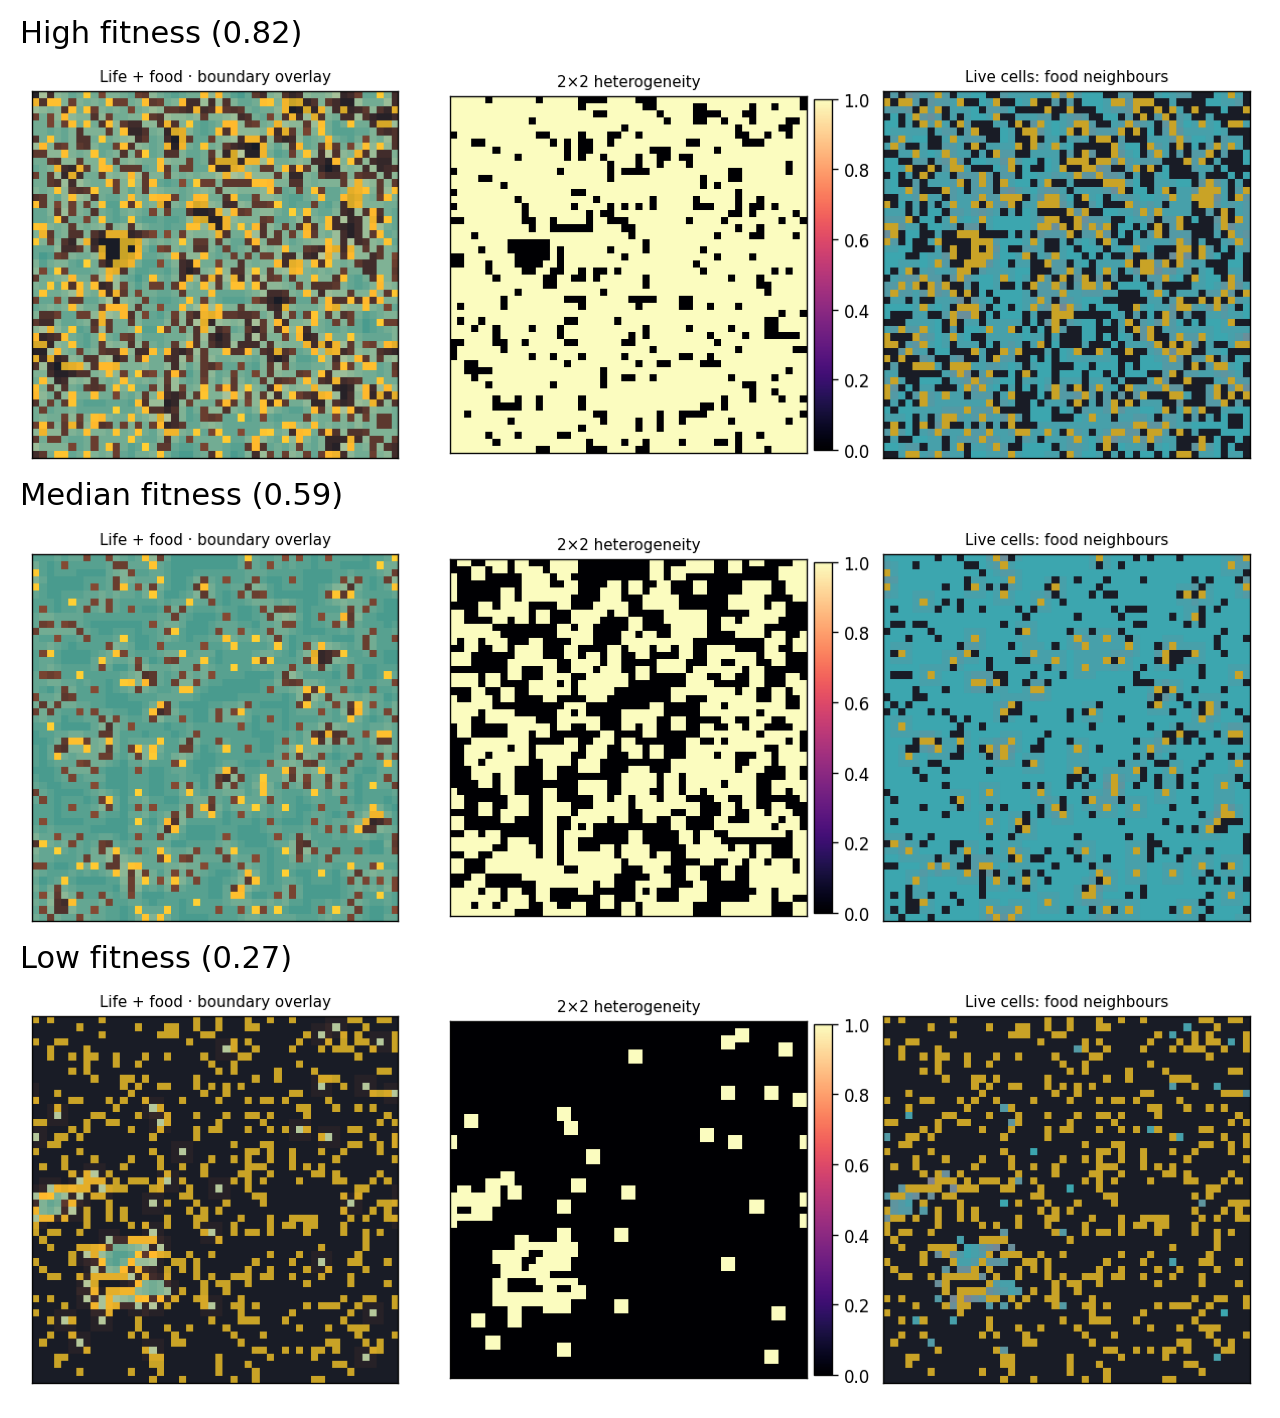
\includegraphics[width=\linewidth,height=0.82\textheight,keepaspectratio]{fig02_elite_worlds.png}
  \caption{Example elites from \texttt{hints}, seed~4 (\texttt{q1-full}): high, median, and low fitness in the 50$\times$50 behaviour archive (10th / 50th / max rank among filled cells; fitness labels from collapsed archive, panels re-simulated via \texttt{run\_world}). Each row shows life--food boundary, 2$\times$2 heterogeneity, and food-neighbour panels for one elite.}
  \label{fig:elites}
\end{figure}

\section{Condition label map}
\label{sec:arm-map}

Internal scheduler / artifact labels (left) are mapped to plain descriptions used in prose.

\begin{table}[!htbp]
  \centering
  \caption{Arm-label map (appendix).}
  \label{tab:arm-map}
  \small
  \fitcenter{%
  \begin{tabular}{@{}llp{5.8cm}@{}}
    \toprule
    Label & Plain name & Meaning \\
    \midrule
    \texttt{stub} & LLM + constant placeholders & Historical control; \texttt{min\_fitness\_frontier} \\
    \texttt{hints} & LLM + live scalar hints & Bundled treatment; \texttt{uniform\_frontier} \\
    \texttt{stub\_uniform} & LLM + constants (matched policy) & Same target selection as \texttt{hints}; surrogate off \\
    \texttt{filter} & LLM + scalars + acquisition & Skip low-acquisition proposals \\
    \texttt{genetic\_me\_uniform} & Genetic ME (matched policy) & No LLM; \texttt{uniform\_frontier} \\
    \texttt{genetic\_me\_filter} & Genetic ME + acquisition & No LLM; threshold filter \\
    \texttt{vanilla} & Random-only ME & 50$\times$ random emitters \\
    \texttt{cma\_me} / \texttt{cma\_mae} & pyribs CMA-ME / CMA-MAE & Continuous ES baselines \\
    \bottomrule
  \end{tabular}%
  }
\end{table}

\section{Repository analysis IDs (appendix only)}
\label{sec:protocol-crosswalk}

Main-text contrasts use only \textbf{H1}--\textbf{H5} (Table~\ref{tab:role-exp}). Frozen analysis scripts and Holm JSON in the repository still use internal ID strings. Table~\ref{tab:families} maps each H-label to those IDs for reproducibility; they are \emph{not} reader-facing names.

\begin{table}[!htbp]
  \centering
  \caption{Repository analysis IDs (appendix only): H-label $\rightarrow$ locked protocol string, Holm width $m$, and outcome ($\alpha=0.05$, Holm within set). Rows marked $^\dagger$ are stack tests with mixed \texttt{target\_selection}; matched H1 is Table~\ref{tab:decomposition}.}
  \label{tab:rq-map}
  \label{tab:families}
  \small
  \fitcenter{%
  \begin{tabular}{@{}llp{2.8cm}cl@{}}
    \toprule
    H-label / check & Locked contrast & Repo analysis ID & $m$ & Outcome \\
    \midrule
    H1 (before-gen) & \texttt{stub\_uniform} vs.\ \texttt{hints} & \emph{not} F-RQ1 & --- & exploratory; TOST$\pm$2~pp accept \\
    Shared-checkpoint gate & Hold-out $R^2$/MAE & \texttt{hints\_ok} & --- & PASS \\
    H2 (after-gen) & \texttt{genetic\_me\_uniform} vs.\ \texttt{genetic\_me\_filter} & primary-grid matched-eval & --- & eval-eff.\ gain (not terminal/wall) \\
    H3 (interaction) & \texttt{hints} vs.\ \texttt{filter} & compose-gate fail (diagnosed) & --- & exploratory; gray-zone repair deferred \\
    H4 (ceiling) & hints $>$ cma\_me \textbf{and} hints $>$ cma\_mae & F-RQ-ceiling (\texttt{F-RQ4}) & 4 & does not pass \\
    H5 (transfer) & dungeon AUC (filter, hints, interaction) & F-B4-dungeon & 8 & partial \\
    H5 (maze interim) & maze AUC (same contrasts) & F-B5-maze & 8 & interim $n{=}5$; CPU $n{=}10$ H2 passes \\
    Bundled confound$^\dagger$ & hints $>$ stub ($\Delta$cov \& $\Delta$fit) & F-RQ1 & 2 & passes$^\dagger$ (not H1) \\
    Bundled floor$^\dagger$ & hints $>$ vanilla ($\Delta$cov \& $\Delta$fit) & F-RQ0 & 2 & passes$^\dagger$ \\
    Multi-provider$^\dagger$ & hints $>$ stub \emph{per} LLM & F-RQ1g & $2$/model & passes$^\dagger$ (same confound) \\
    Geometry robustness & Grid vs.\ CVT & appendix only & --- & descriptive \\
    \bottomrule
  \end{tabular}%
  }
\end{table}

\begin{table}[!htbp]
  \centering
  \caption{Paper-wide Holm robustness ($\alpha{=}0.05$, $m{=}20$): one step-down over all locked confirmatory raw $p$-values. Primary claims remain within-set (Table~\ref{tab:families}). Within-set and paper-wide reject columns agree on every row that drives a pass/fail outcome; dungeon hints$-$stub AUC tests remain non-rejects under both corrections. Column~1 keeps repository analysis IDs for artifact matching.}
  \label{tab:paper-holm}
  \scriptsize
  \fitcenter{%
  \begin{tabular}{@{}llp{4.6cm}rcc@{}}
    \toprule
    Repo ID & Contrast & Raw $p$ & Within-set & Paper-wide \\
    \midrule
    bundled stack & hints $>$ stub coverage & $9.8\times10^{-4}$ & Yes & Yes \\
    bundled stack & hints $>$ stub fitness & $9.8\times10^{-4}$ & Yes & Yes \\
    bundled floor & hints $>$ vanilla coverage & $9.8\times10^{-4}$ & Yes & Yes \\
    bundled floor & hints $>$ vanilla fitness & $9.8\times10^{-4}$ & Yes & Yes \\
    H4 & hints $>$ cma\_mae fitness & $9.8\times10^{-4}$ & Yes & Yes \\
    H4 & hints $>$ cma\_mae coverage & $0.50$ & No & No \\
    H4 & hints $>$ cma\_me coverage & $1.0$ & No & No \\
    H4 & hints $>$ cma\_me fitness & $1.0$ & No & No \\
    H5 dungeon & genetic\_filter $-$ genetic cov.\ AUC & $9.8\times10^{-4}$ & Yes & Yes \\
    H5 dungeon & genetic\_filter $-$ genetic QD AUC & $9.8\times10^{-4}$ & Yes & Yes \\
    H5 dungeon & hints $-$ stub QD AUC & $0.019$ & No & No \\
    H5 dungeon & hints $-$ stub cov.\ AUC & $0.032$ & No & No \\
    H5 dungeon & LLM filter $-$ hints cov.\ AUC & $0.50$ & No & No \\
    H5 dungeon & LLM filter $-$ hints QD AUC & $0.69$ & No & No \\
    H5 dungeon & acquisition interaction cov.\ AUC & $1.0$ & No & No \\
    H5 dungeon & acquisition interaction QD AUC & $1.0$ & No & No \\
    multi-prov.\ DeepSeek & hints $>$ stub coverage & $9.8\times10^{-4}$ & Yes & Yes \\
    multi-prov.\ DeepSeek & hints $>$ stub fitness & $9.8\times10^{-4}$ & Yes & Yes \\
    multi-prov.\ gpt-4o-mini & hints $>$ stub coverage & $9.8\times10^{-4}$ & Yes & Yes \\
    multi-prov.\ gpt-4o-mini & hints $>$ stub fitness & $2.9\times10^{-3}$ & Yes & Yes \\
    \bottomrule
  \end{tabular}%
  }
\end{table}

\noindent\textit{Readout:} $11/20$ paper-wide rejects. Bundled stack, floor, multi-provider, and dungeon H2 AUC transfers still reject after the global correction; H4 and the non-transfer dungeon contrasts remain non-rejects. Exact repository strings (\texttt{F-RQ*}, \texttt{F-B4-*}) are in Table~\ref{tab:families}. Artifact: \texttt{artifacts/experiments/paper\_wide\_holm\_robustness.json}.

\section{Per-seed paired deltas (bundled stack)}

\begin{table}[!htbp]
  \centering
  \caption{Bundled stack per-seed levels and paired hints $-$ stub ($n=10$; same contrast as Table~\ref{tab:rq1}).}
  \label{tab:rq1-seeds}
  \small
  \fitcenter{%
  \begin{tabular}{@{}rrrrrrr@{}}
    \toprule
    Seed & Stub cov (\%) & Hints cov (\%) & $\Delta$cov & Stub fit & Hints fit & $\Delta$fit \\
    \midrule
    0 & 43.72 & 59.72 & $+16.00$ & 0.446 & 0.498 & $+0.052$ \\
    1 & 46.08 & 59.24 & $+13.16$ & 0.455 & 0.500 & $+0.046$ \\
    2 & 42.88 & 61.00 & $+18.12$ & 0.438 & 0.488 & $+0.050$ \\
    3 & 44.32 & 61.60 & $+17.28$ & 0.449 & 0.506 & $+0.057$ \\
    4 & 43.36 & 60.48 & $+17.12$ & 0.443 & 0.501 & $+0.059$ \\
    5 & 44.24 & 60.52 & $+16.28$ & 0.445 & 0.498 & $+0.054$ \\
    6 & 50.60 & 61.16 & $+10.56$ & 0.477 & 0.505 & $+0.028$ \\
    7 & 44.56 & 59.12 & $+14.56$ & 0.449 & 0.493 & $+0.044$ \\
    8 & 48.48 & 60.80 & $+12.32$ & 0.468 & 0.498 & $+0.030$ \\
    9 & 44.92 & 60.44 & $+15.52$ & 0.455 & 0.501 & $+0.046$ \\
    \bottomrule
  \end{tabular}%
  }
\end{table}

\section{CVT archive sensitivity}
\label{sec:cvt-sensitivity}

The scientific object of this paper is the attachment-point split (H1 / H2) on the confirmatory $50\times50$ grid (with H3 only as a descriptive LLM-stack check), not archive geometry. A CVT sensitivity run (\texttt{q1-cvt}, $n{=}10$) only checks that the \emph{bundled} stub/hints/filter directions are not grid-specific (Table~\ref{tab:cvt}): H1-s concordance 10/10; H3-s evaluation reduction $\sim$31\% on CVT vs.\ 33.5\% on grid. Absolute $\Delta$coverage is larger on CVT mainly because the stub baseline is lower ($\sim$37\% vs.\ $\sim$45\%). These runs are descriptive and outside confirmatory Holm contrast sets; they do not alter the H1 flat matched contrast or H2 eval-axis claims.

\begin{table}[!htbp]
  \centering
  \caption{CVT sensitivity only (paired $n=10$; not confirmatory).}
  \label{tab:cvt}
  \small
  \fitcenter{%
  \begin{tabular}{@{}lrrrr@{}}
    \toprule
    Archive & H1-s $\Delta$cov (pp) & H1-s sign & H3-s eval$\downarrow$ & Stub cov (\%) \\
    \midrule
    Grid (confirmatory) & $+15.09 \pm 2.42$ & 10/10 & 33.5\% & $45.3 \pm 2.4$ \\
    CVT (sensitivity) & $+21.51 \pm 0.79$ & 10/10 & 30.8\% & $37.4 \pm 0.4$ \\
    \bottomrule
  \end{tabular}%
  }
\end{table}

\section{Archive heatmap panel (supplemental)}
\label{sec:heatmap-panel}

Paired hints vs.\ CMA-ME archive fitness heatmaps for seeds~1, 4, and 6 (collapsed warm-start archives; same colour scale and layout as main-text Figure~\ref{fig:heatmaps}). Seed~4 is the main-text panel ($\Delta$cov $-20.0$~pp); seeds~1 and~6 illustrate smaller and mid-large paired gaps ($-9.4$ / $-16.0$~pp).

\begin{figure}[!htbp]
  \centering
  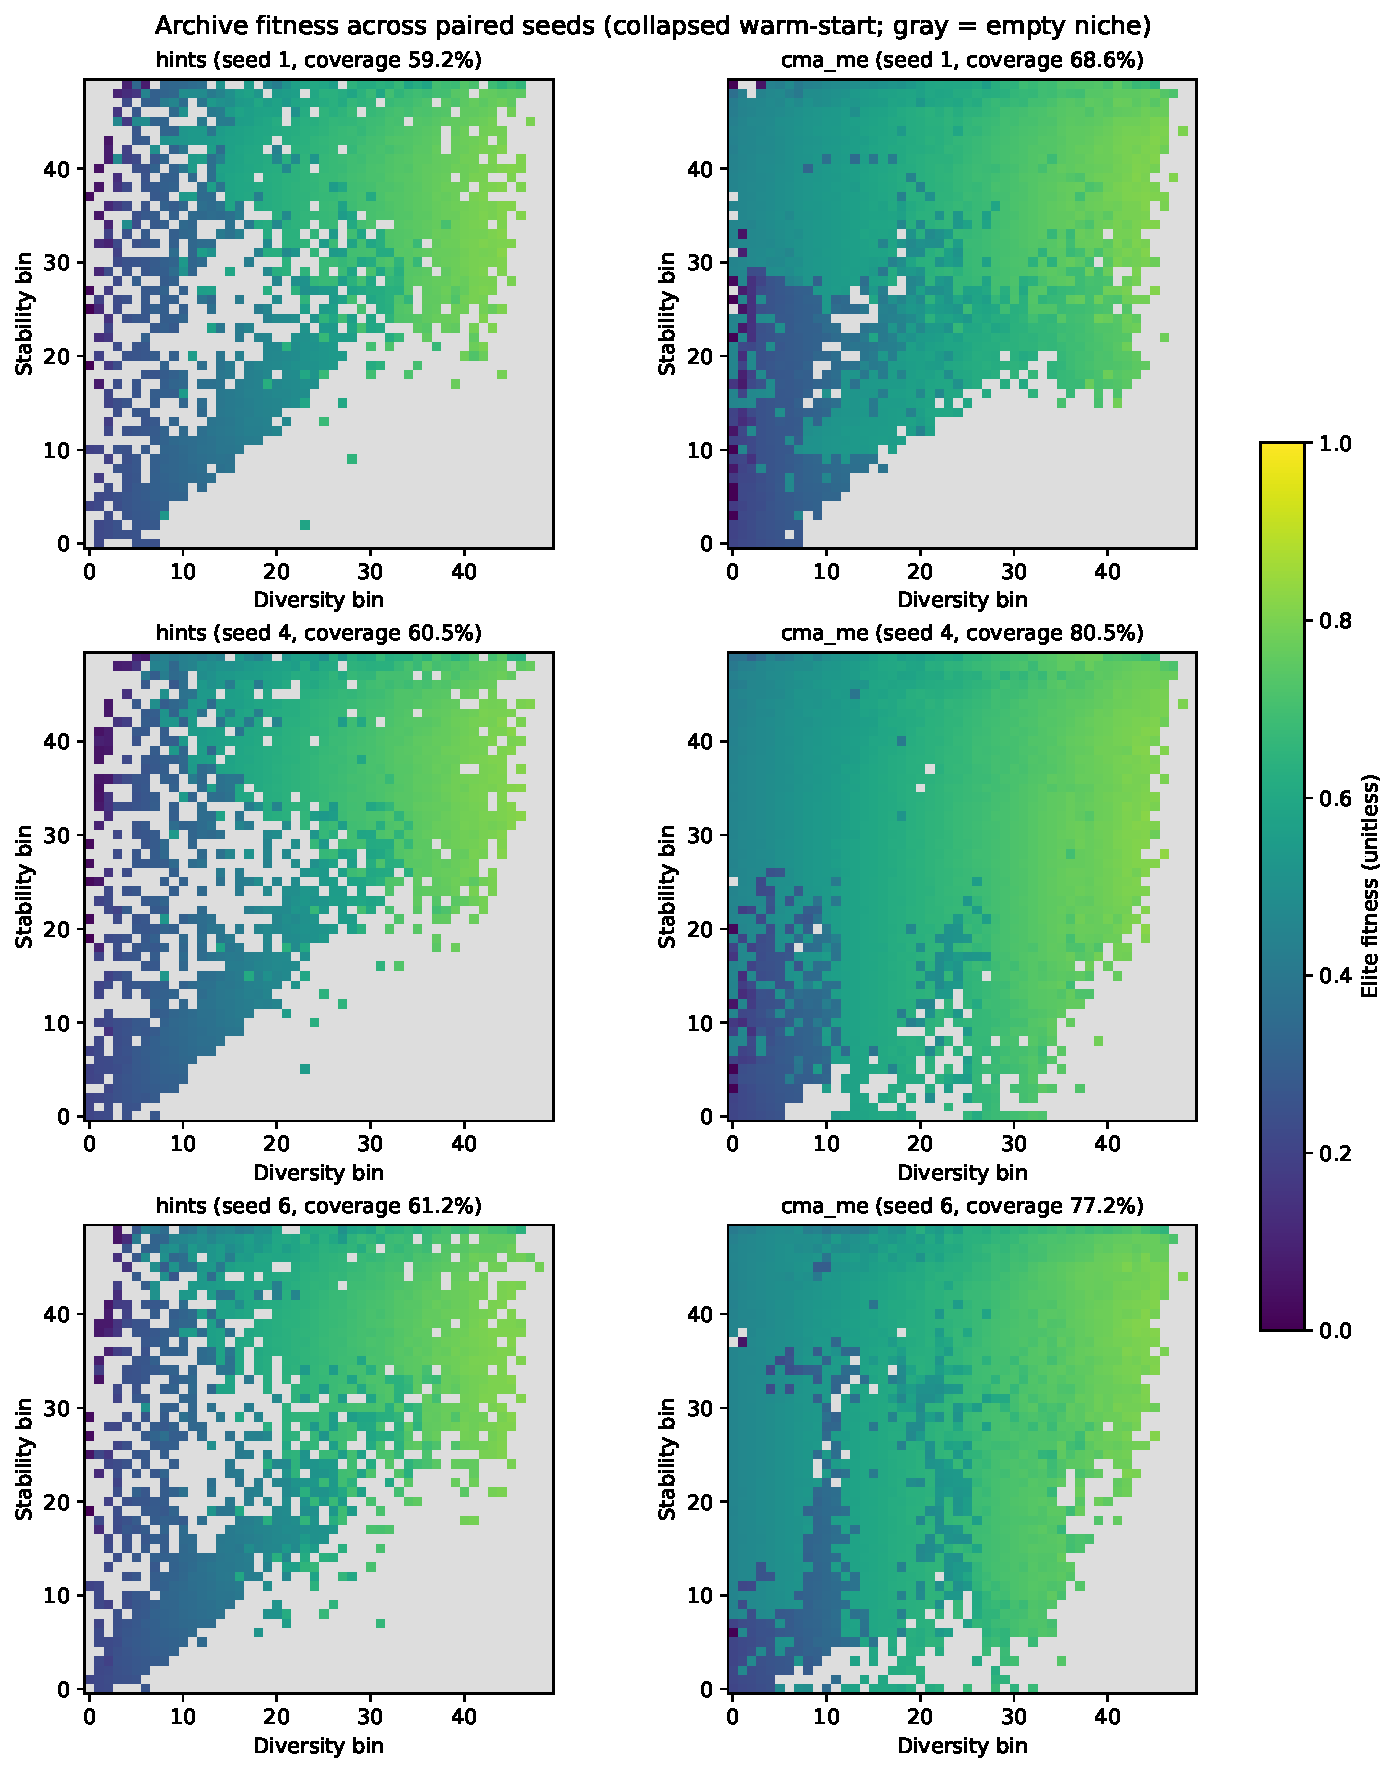
\includegraphics[width=\linewidth]{fig07_archive_heatmaps_panel_seeds1_4_6.pdf}
  \caption{Supplemental archive heatmaps: hints vs.\ CMA-ME for paired seeds~1, 4, and~6 (\texttt{q1-full} / \texttt{q1-v3-pyribs}). Rows = seed; columns = hints (left) and CMA-ME (right).}
  \label{fig:heatmap-panel}
\end{figure}


\end{document}
